% Options for packages loaded elsewhere
\PassOptionsToPackage{unicode}{hyperref}
\PassOptionsToPackage{hyphens}{url}
%
\documentclass[
]{article}
\usepackage{amsmath,amssymb}
\usepackage{lmodern}
\usepackage{iftex}
\ifPDFTeX
  \usepackage[T1]{fontenc}
  \usepackage[utf8]{inputenc}
  \usepackage{textcomp} % provide euro and other symbols
\else % if luatex or xetex
  \usepackage{unicode-math}
  \defaultfontfeatures{Scale=MatchLowercase}
  \defaultfontfeatures[\rmfamily]{Ligatures=TeX,Scale=1}
\fi
% Use upquote if available, for straight quotes in verbatim environments
\IfFileExists{upquote.sty}{\usepackage{upquote}}{}
\IfFileExists{microtype.sty}{% use microtype if available
  \usepackage[]{microtype}
  \UseMicrotypeSet[protrusion]{basicmath} % disable protrusion for tt fonts
}{}
\makeatletter
\@ifundefined{KOMAClassName}{% if non-KOMA class
  \IfFileExists{parskip.sty}{%
    \usepackage{parskip}
  }{% else
    \setlength{\parindent}{0pt}
    \setlength{\parskip}{6pt plus 2pt minus 1pt}}
}{% if KOMA class
  \KOMAoptions{parskip=half}}
\makeatother
\usepackage{xcolor}
\usepackage[margin=1in]{geometry}
\usepackage{graphicx}
\makeatletter
\def\maxwidth{\ifdim\Gin@nat@width>\linewidth\linewidth\else\Gin@nat@width\fi}
\def\maxheight{\ifdim\Gin@nat@height>\textheight\textheight\else\Gin@nat@height\fi}
\makeatother
% Scale images if necessary, so that they will not overflow the page
% margins by default, and it is still possible to overwrite the defaults
% using explicit options in \includegraphics[width, height, ...]{}
\setkeys{Gin}{width=\maxwidth,height=\maxheight,keepaspectratio}
% Set default figure placement to htbp
\makeatletter
\def\fps@figure{htbp}
\makeatother
\setlength{\emergencystretch}{3em} % prevent overfull lines
\providecommand{\tightlist}{%
  \setlength{\itemsep}{0pt}\setlength{\parskip}{0pt}}
\setcounter{secnumdepth}{-\maxdimen} % remove section numbering
\usepackage{booktabs}
\usepackage{sectsty} \allsectionsfont{\centering\huge}
\usepackage{sectsty} \subsectionfont{\centering\LARGE}
\usepackage{sectsty} \subsubsectionfont{\centering\Large}
\usepackage{sectsty} \paragraphfont{\large}
\usepackage{sectsty} \subparagraphfont{\normalsize}
\usepackage{titlesec}
\usepackage{lipsum}
\usepackage{booktabs}
\usepackage{longtable}
\usepackage{array}
\usepackage{multirow}
\usepackage{wrapfig}
\usepackage{float}
\usepackage{colortbl}
\usepackage{pdflscape}
\usepackage{tabu}
\usepackage{threeparttable}
\usepackage{threeparttablex}
\usepackage[normalem]{ulem}
\usepackage{makecell}
\usepackage{xcolor}
\ifLuaTeX
  \usepackage{selnolig}  % disable illegal ligatures
\fi
\IfFileExists{bookmark.sty}{\usepackage{bookmark}}{\usepackage{hyperref}}
\IfFileExists{xurl.sty}{\usepackage{xurl}}{} % add URL line breaks if available
\urlstyle{same} % disable monospaced font for URLs
\hypersetup{
  pdftitle={Hippocampal subfield},
  pdfauthor={Daniela Cossio},
  hidelinks,
  pdfcreator={LaTeX via pandoc}}

\title{Hippocampal subfield}
\author{Daniela Cossio}
\date{08 October 2024}

\begin{document}
\maketitle

{
\setcounter{tocdepth}{3}
\tableofcontents
}
\newpage

\section{Methods}

\vspace{1cm}
\vspace{1cm}

\section{Results}
\vspace{1cm}
\subsection{Angular Error}
\vspace{1cm}

\subsubsection{Average}

Total N= 27 F=16 M=11

\paragraph{CA1}

~ There were no significant associations between CA1 and average angular
error across men and women. ( Correlations are not controlled by sex.)
All linear regressions run with a pearson \vspace{1cm}

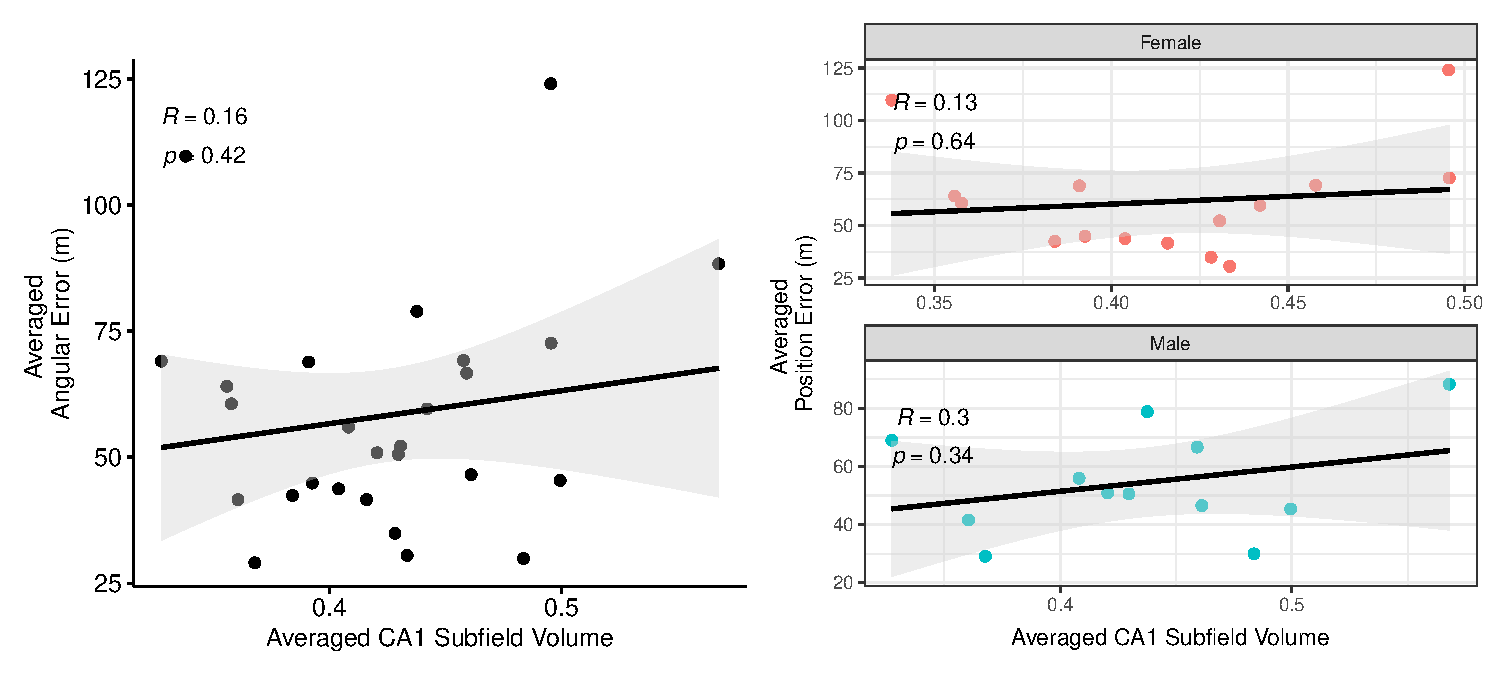
\includegraphics{hippocampal_subfield_files/figure-latex/unnamed-chunk-1-1.pdf}

\vspace{1cm}

Running multiple linear regressions to see the effect of age and sex and
then plotting results

\begin{verbatim}
## 
## Call:
## lm(formula = loop_ae_avg_degree ~ t2hipp_vol_avg_ca1 + age_spatial_years + 
##     sex, data = df)
## 
## Residuals:
##     Min      1Q  Median      3Q     Max 
## -32.249 -15.502  -3.172   8.604  56.596 
## 
## Coefficients:
##                     Estimate Std. Error t value Pr(>|t|)
## (Intercept)         22.94464  124.46691   0.184    0.855
## t2hipp_vol_avg_ca1  82.20637  105.06111   0.782    0.442
## age_spatial_years    0.08383    1.85054   0.045    0.964
## sexMale             -8.48312    9.28906  -0.913    0.371
## 
## Residual standard error: 23.57 on 23 degrees of freedom
##   (1 observation deleted due to missingness)
## Multiple R-squared:  0.05989,    Adjusted R-squared:  -0.06273 
## F-statistic: 0.4884 on 3 and 23 DF,  p-value: 0.6937
\end{verbatim}

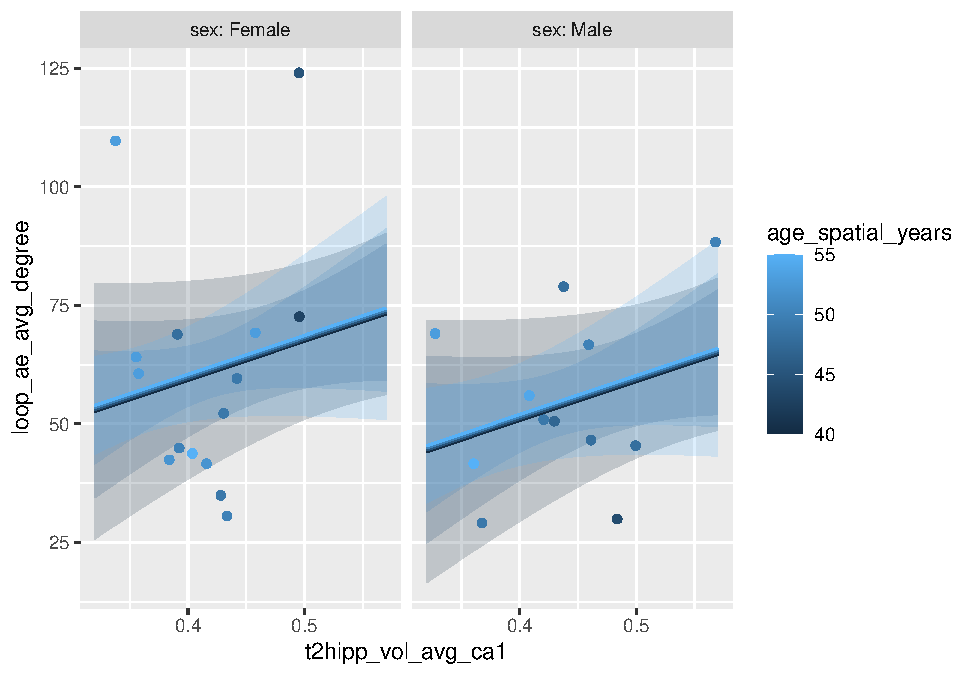
\includegraphics{hippocampal_subfield_files/figure-latex/Avg CA1 + avg angular error MLR-1.pdf}

\newpage
\paragraph{CA2/3}

\subparagraph{There were no significant associations between CA2/3 and average angular error across men and women. The lm was run using a pearson. When conducting the sex stratification, men were analyzed using a spearman and women with a pearson}

~ \vspace{1cm}

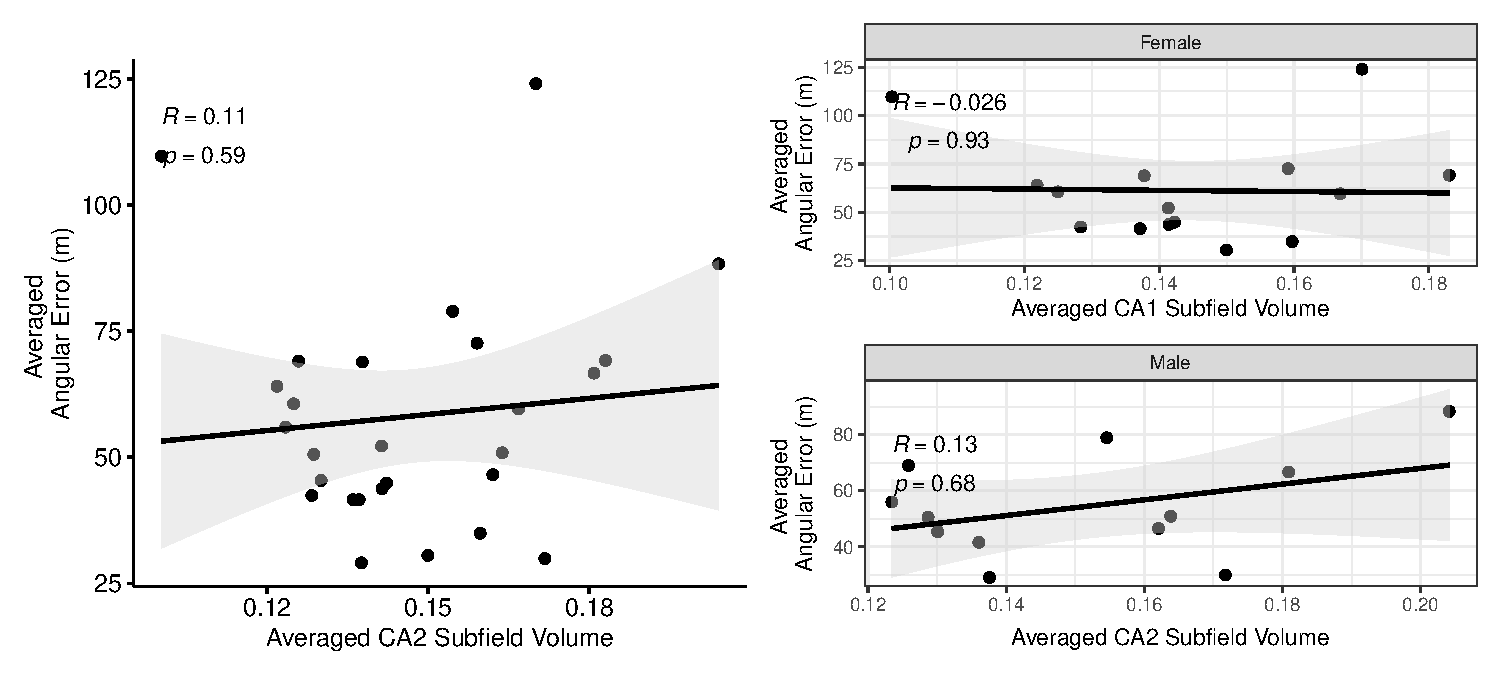
\includegraphics{hippocampal_subfield_files/figure-latex/unnamed-chunk-2-1.pdf}

\vspace{1cm}

Running multiple linear regressions to see the effect of age and sex and
then plotting results

\begin{verbatim}
## 
## Call:
## lm(formula = loop_ae_avg_degree ~ t2hipp_vol_avg_ca23 + age_spatial_years + 
##     sex, data = df)
## 
## Residuals:
##     Min      1Q  Median      3Q     Max 
## -31.471 -15.632  -4.712   6.959  57.519 
## 
## Coefficients:
##                     Estimate Std. Error t value Pr(>|t|)
## (Intercept)          69.5909    99.6115   0.699    0.492
## t2hipp_vol_avg_ca23 107.3413   223.8324   0.480    0.636
## age_spatial_years    -0.4739     1.6271  -0.291    0.773
## sexMale              -7.9649     9.3353  -0.853    0.402
## 
## Residual standard error: 23.77 on 23 degrees of freedom
##   (1 observation deleted due to missingness)
## Multiple R-squared:  0.04442,    Adjusted R-squared:  -0.08022 
## F-statistic: 0.3564 on 3 and 23 DF,  p-value: 0.785
\end{verbatim}

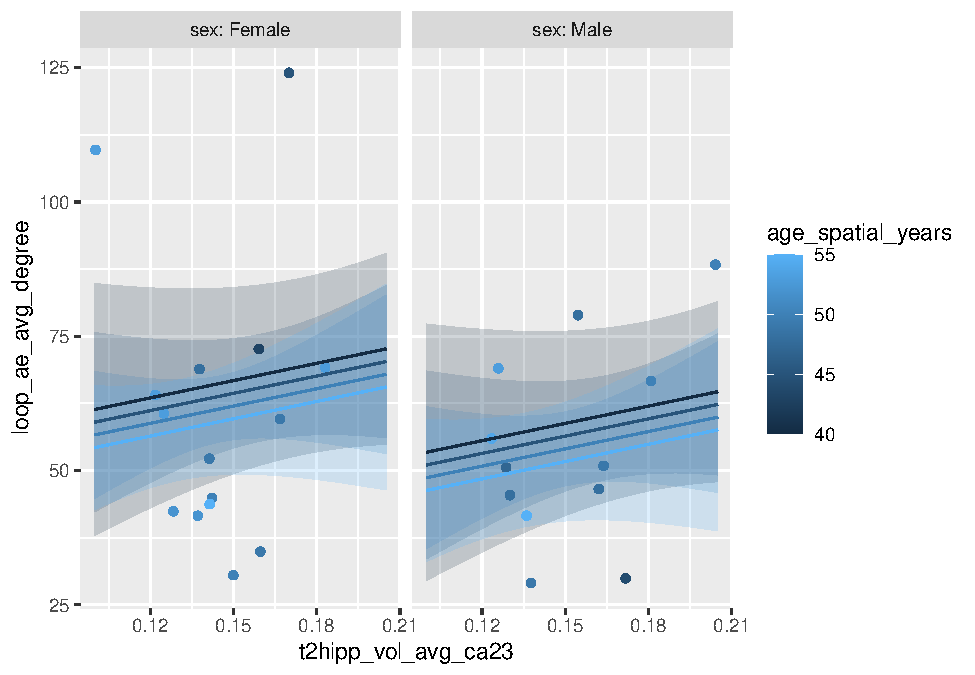
\includegraphics{hippocampal_subfield_files/figure-latex/Avg CA2 + avg angular error MLR-1.pdf}

\paragraph{DG}

~ \vspace{1cm}

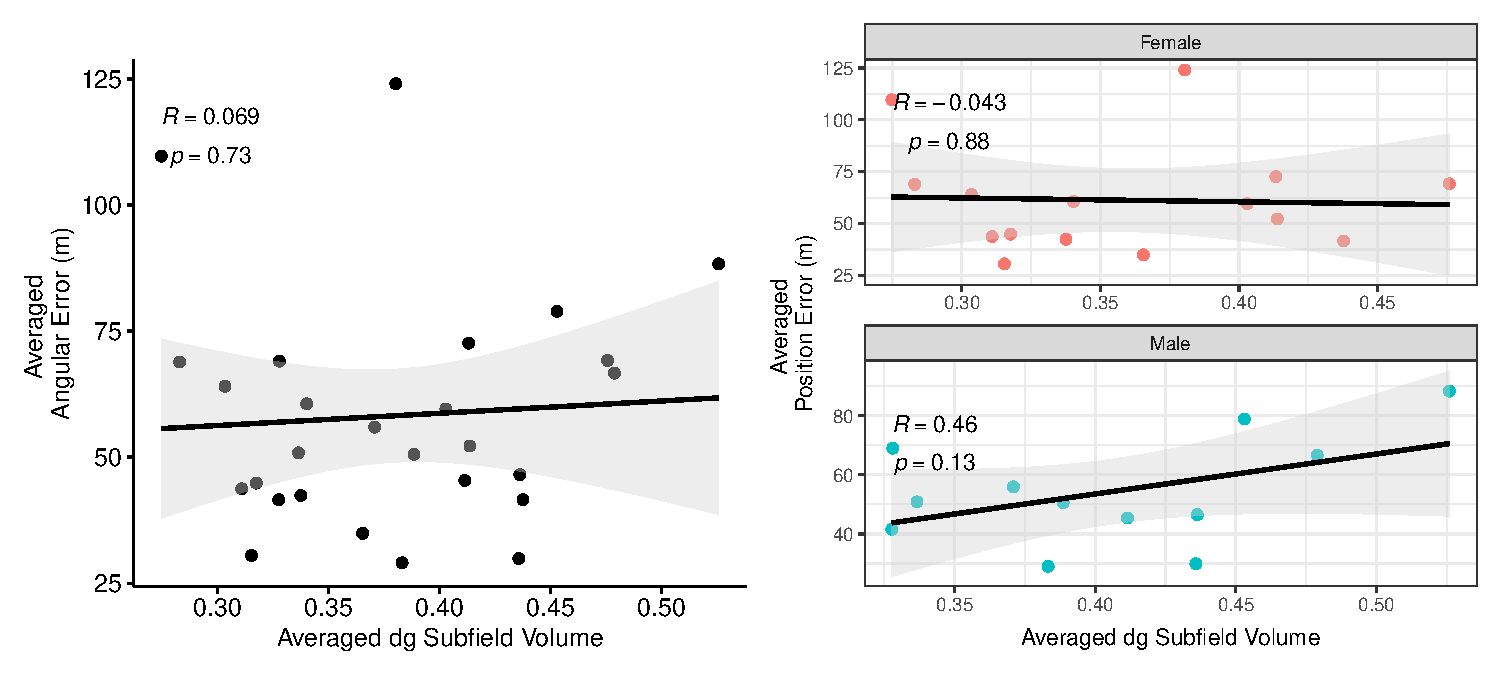
\includegraphics{hippocampal_subfield_files/figure-latex/unnamed-chunk-3-1.pdf}

\vspace{1cm}

Running multiple linear regressions to see the effect of age and sex and
then plotting results

\begin{verbatim}
## 
## Call:
## lm(formula = loop_ae_avg_degree ~ t2hipp_vol_avg_dg + age_spatial_years + 
##     sex, data = df)
## 
## Residuals:
##     Min      1Q  Median      3Q     Max 
## -29.044 -13.924  -4.257   7.967  59.117 
## 
## Coefficients:
##                   Estimate Std. Error t value Pr(>|t|)
## (Intercept)        71.9035    93.6438   0.768    0.450
## t2hipp_vol_avg_dg  42.7105    82.3755   0.518    0.609
## age_spatial_years  -0.5161     1.5770  -0.327    0.746
## sexMale            -9.2691     9.9309  -0.933    0.360
## 
## Residual standard error: 23.75 on 23 degrees of freedom
##   (1 observation deleted due to missingness)
## Multiple R-squared:  0.04601,    Adjusted R-squared:  -0.07842 
## F-statistic: 0.3698 on 3 and 23 DF,  p-value: 0.7755
\end{verbatim}

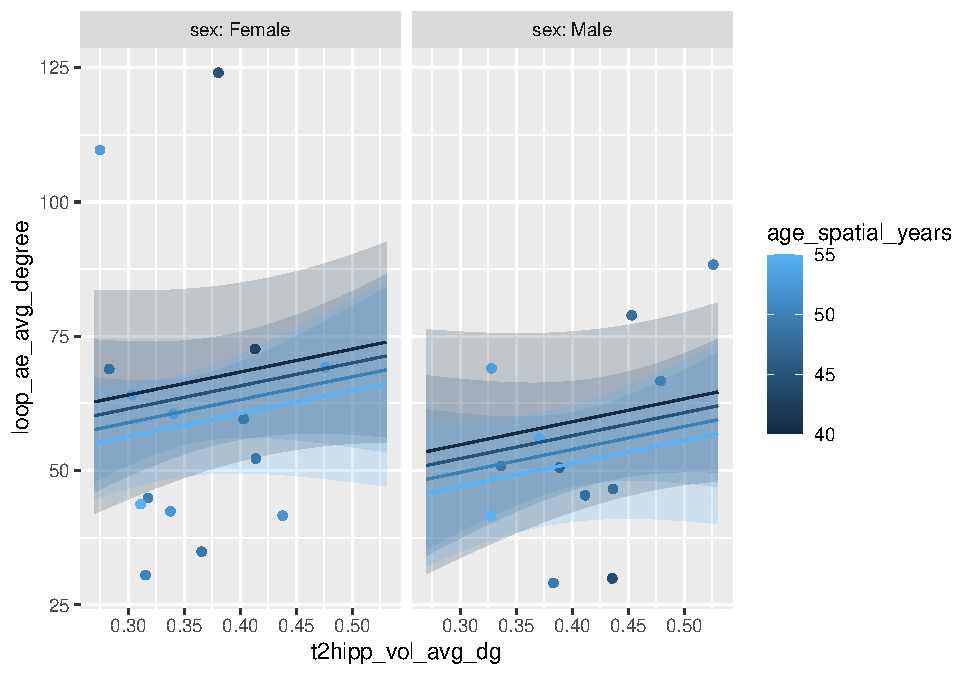
\includegraphics{hippocampal_subfield_files/figure-latex/Avg DG + avg angular error MLR-1.pdf}

\newpage
\paragraph{PHC}

~ \vspace{1cm}

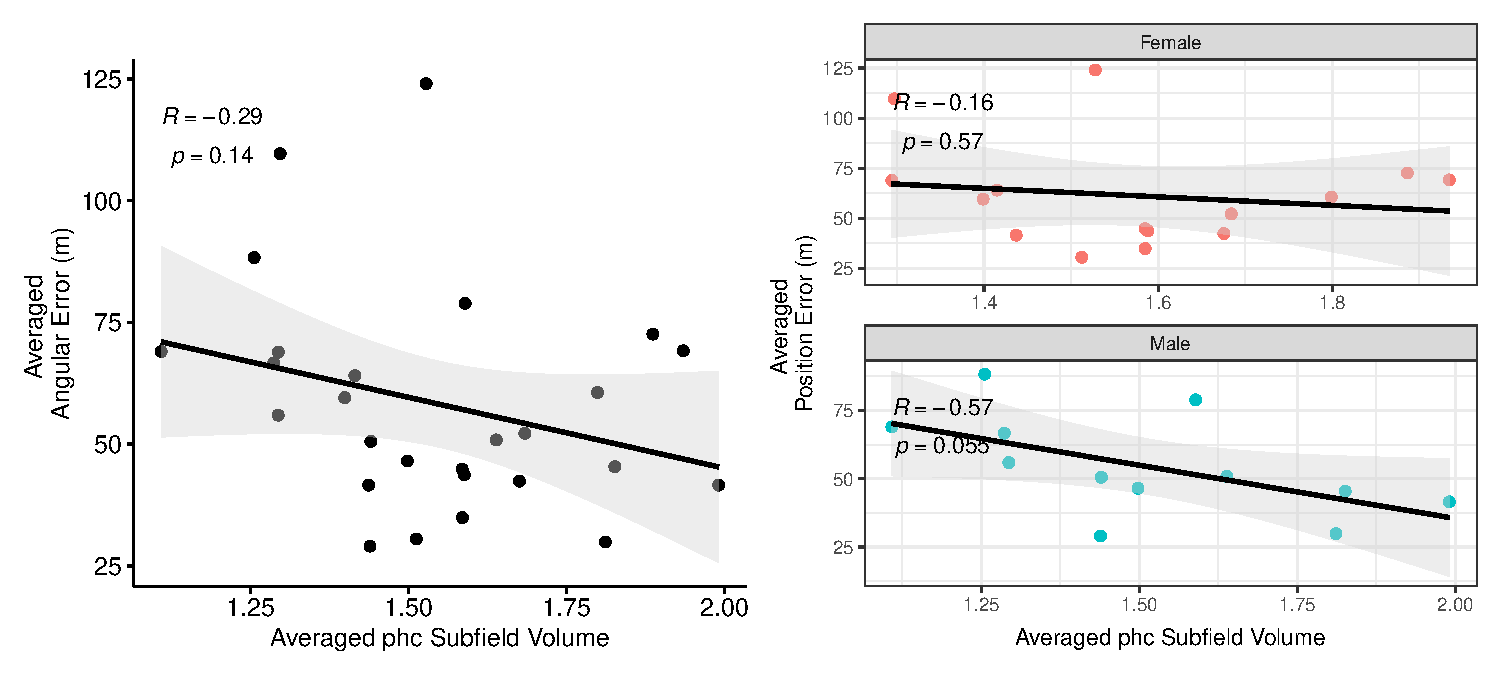
\includegraphics{hippocampal_subfield_files/figure-latex/unnamed-chunk-4-1.pdf}

\vspace{1cm}

Running multiple linear regressions to see the effect of age and sex and
then plotting results

\begin{verbatim}
## 
## Call:
## lm(formula = loop_ae_avg_degree ~ t2hipp_vol_avg_phc + age_spatial_years + 
##     sex, data = df)
## 
## Residuals:
##     Min      1Q  Median      3Q     Max 
## -33.200 -12.366  -0.796  10.158  54.904 
## 
## Coefficients:
##                    Estimate Std. Error t value Pr(>|t|)  
## (Intercept)         175.273     82.770   2.118   0.0452 *
## t2hipp_vol_avg_phc  -34.412     19.858  -1.733   0.0965 .
## age_spatial_years    -1.190      1.423  -0.836   0.4115  
## sexMale              -9.727      8.855  -1.098   0.2834  
## ---
## Signif. codes:  0 '***' 0.001 '**' 0.01 '*' 0.05 '.' 0.1 ' ' 1
## 
## Residual standard error: 22.46 on 23 degrees of freedom
##   (1 observation deleted due to missingness)
## Multiple R-squared:  0.1463, Adjusted R-squared:  0.03497 
## F-statistic: 1.314 on 3 and 23 DF,  p-value: 0.2939
\end{verbatim}

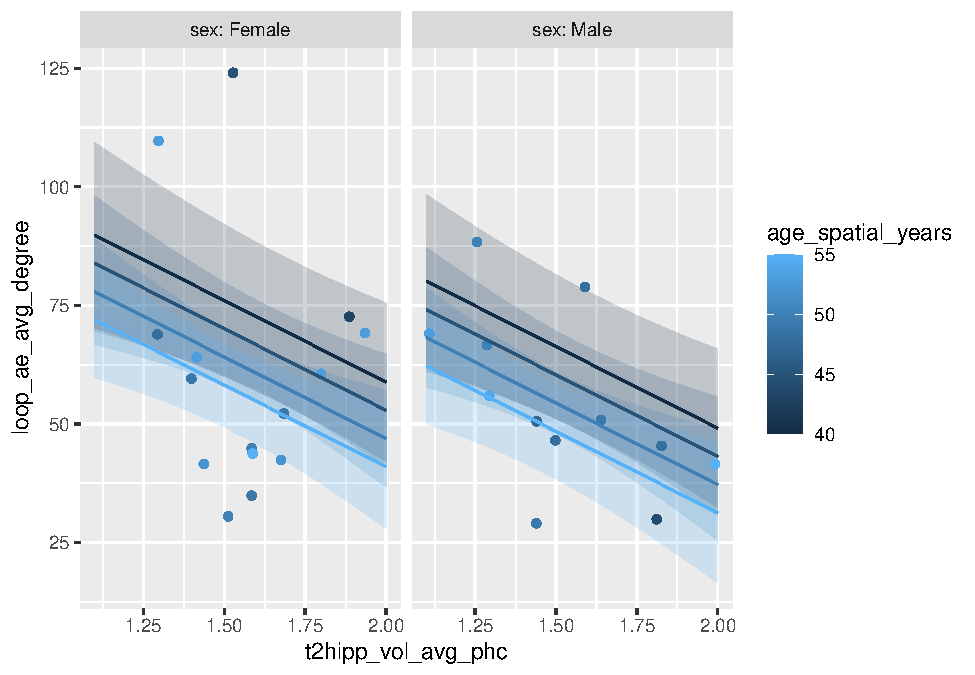
\includegraphics{hippocampal_subfield_files/figure-latex/Avg PHC + avg angular error MLR-1.pdf}

\vspace{1cm}

\paragraph{PRC}

~ \vspace{1cm}

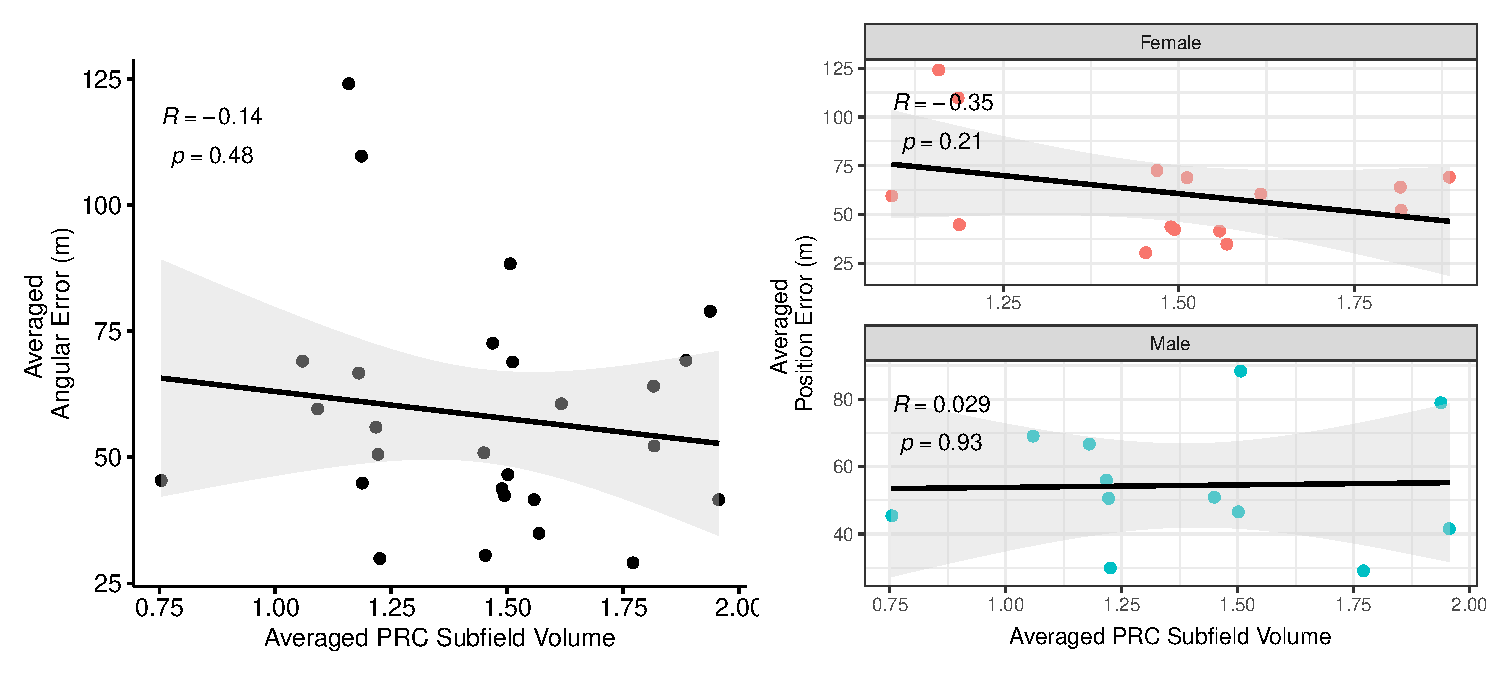
\includegraphics{hippocampal_subfield_files/figure-latex/unnamed-chunk-5-1.pdf}

\vspace{1cm}

Running multiple linear regressions to see the effect of age and sex and
then plotting results

\begin{verbatim}
## 
## Call:
## lm(formula = loop_ae_avg_degree ~ t2hipp_vol_avg_prc + age_spatial_years + 
##     sex, data = df)
## 
## Residuals:
##     Min      1Q  Median      3Q     Max 
## -31.264 -17.531  -3.548   9.012  56.209 
## 
## Coefficients:
##                    Estimate Std. Error t value Pr(>|t|)
## (Intercept)         105.192     74.725   1.408    0.173
## t2hipp_vol_avg_prc  -11.428     16.076  -0.711    0.484
## age_spatial_years    -0.536      1.520  -0.353    0.728
## sexMale              -8.234      9.281  -0.887    0.384
## 
## Residual standard error: 23.63 on 23 degrees of freedom
##   (1 observation deleted due to missingness)
## Multiple R-squared:  0.05561,    Adjusted R-squared:  -0.06757 
## F-statistic: 0.4515 on 3 and 23 DF,  p-value: 0.7187
\end{verbatim}

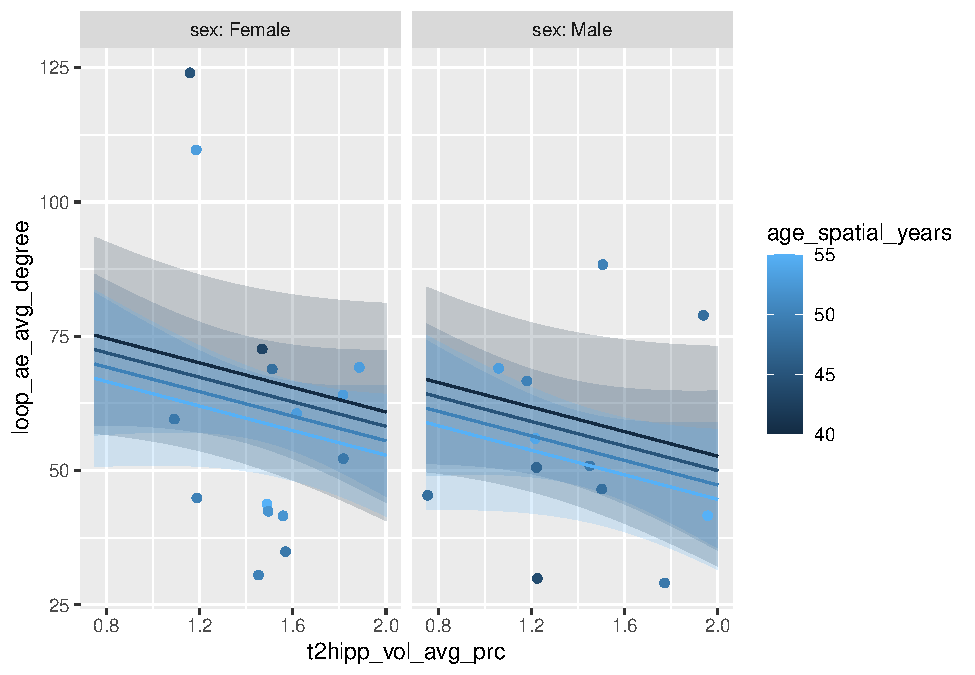
\includegraphics{hippocampal_subfield_files/figure-latex/Avg PRC + avg angular error MLR-1.pdf}
\vspace{1cm}

\newpage
\paragraph{ERC}

~ \vspace{1cm}

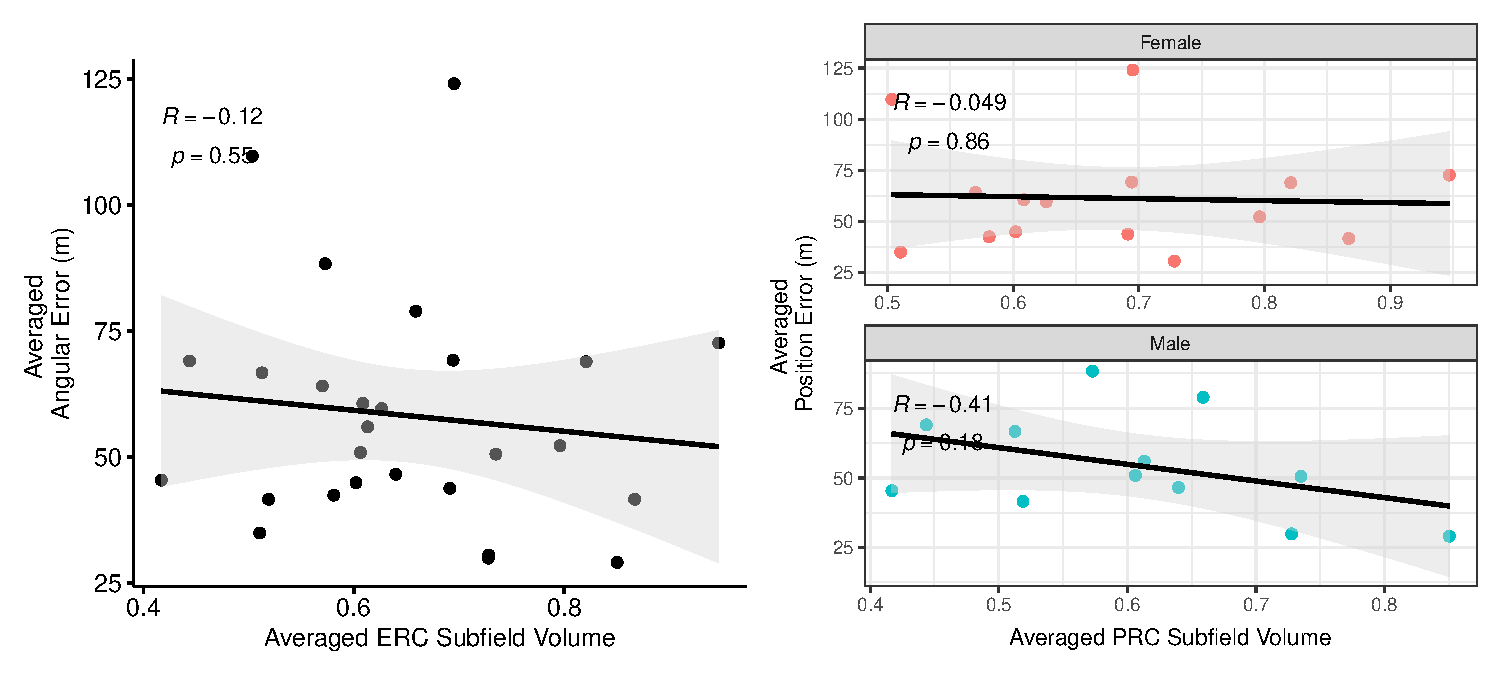
\includegraphics{hippocampal_subfield_files/figure-latex/unnamed-chunk-6-1.pdf}

\vspace{1cm}

Running multiple linear regressions to see the effect of age and sex and
then plotting results

\begin{verbatim}
## 
## Call:
## lm(formula = loop_ae_avg_degree ~ t2hipp_vol_avg_erc + age_spatial_years + 
##     sex, data = df)
## 
## Residuals:
##     Min      1Q  Median      3Q     Max 
## -37.766 -11.320  -4.685  11.449  53.864 
## 
## Coefficients:
##                    Estimate Std. Error t value Pr(>|t|)  
## (Intercept)         188.816     99.616   1.895   0.0707 .
## t2hipp_vol_avg_erc  -52.875     41.015  -1.289   0.2102  
## age_spatial_years    -1.819      1.648  -1.104   0.2809  
## sexMale             -12.055      9.686  -1.245   0.2258  
## ---
## Signif. codes:  0 '***' 0.001 '**' 0.01 '*' 0.05 '.' 0.1 ' ' 1
## 
## Residual standard error: 23.07 on 23 degrees of freedom
##   (1 observation deleted due to missingness)
## Multiple R-squared:  0.0999, Adjusted R-squared:  -0.0175 
## F-statistic: 0.8509 on 3 and 23 DF,  p-value: 0.4804
\end{verbatim}

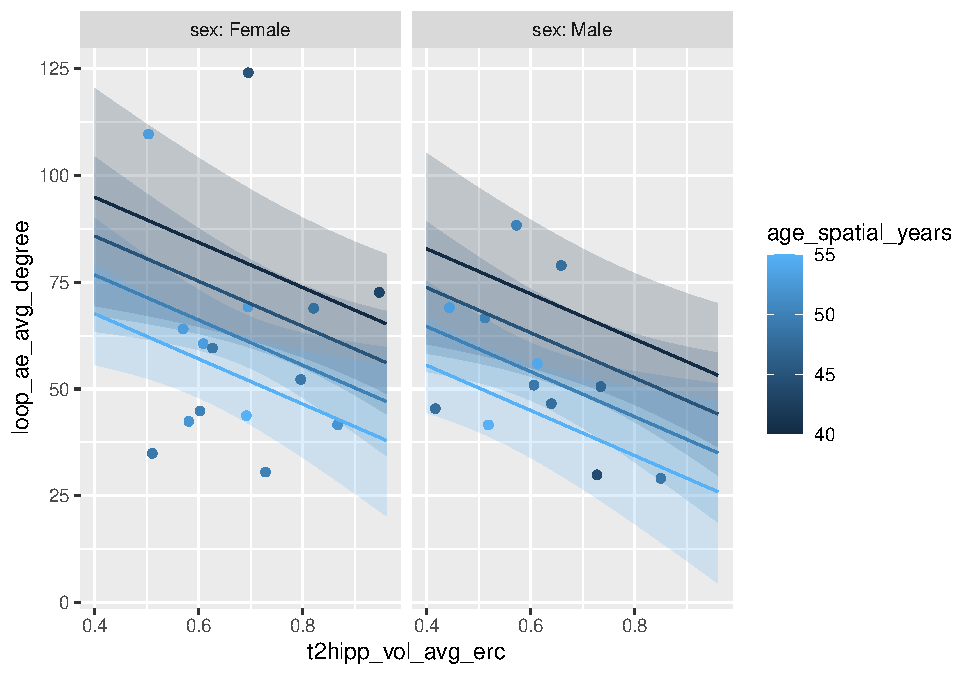
\includegraphics{hippocampal_subfield_files/figure-latex/Avg ERC + avg angular error MLR-1.pdf}
\vspace{1cm}

\paragraph{SUB}

~ \vspace{1cm}

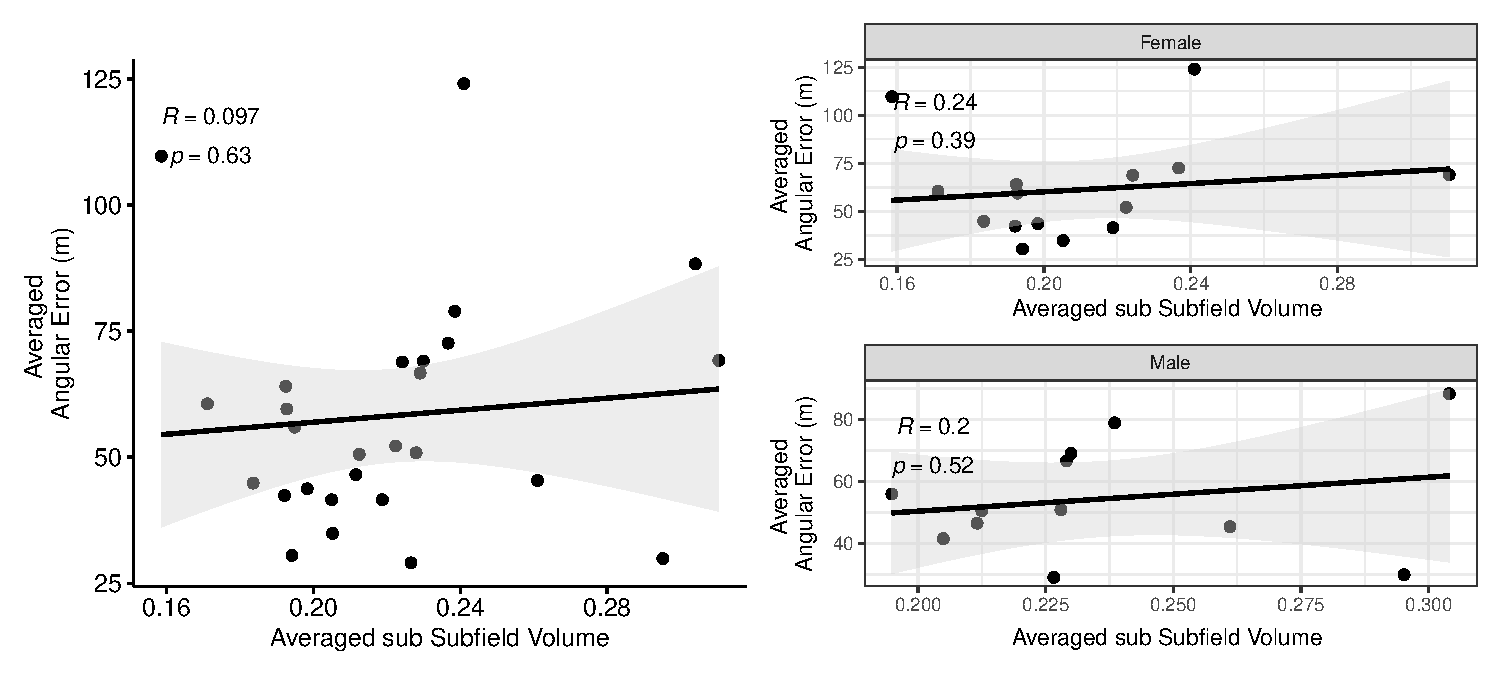
\includegraphics{hippocampal_subfield_files/figure-latex/unnamed-chunk-7-1.pdf}

\vspace{1cm}

Running multiple linear regressions to see the effect of age and sex and
then plotting results

\begin{verbatim}
## 
## Call:
## lm(formula = loop_ae_avg_degree ~ t2hipp_vol_avg_sub + age_spatial_years + 
##     sex, data = df)
## 
## Residuals:
##     Min      1Q  Median      3Q     Max 
## -32.276 -14.312  -2.614   6.561  57.709 
## 
## Coefficients:
##                    Estimate Std. Error t value Pr(>|t|)
## (Intercept)         61.4117    96.1615   0.639    0.529
## t2hipp_vol_avg_sub  94.6134   144.7248   0.654    0.520
## age_spatial_years   -0.3973     1.5979  -0.249    0.806
## sexMale             -9.6746     9.8565  -0.982    0.337
## 
## Residual standard error: 23.67 on 23 degrees of freedom
##   (1 observation deleted due to missingness)
## Multiple R-squared:  0.05247,    Adjusted R-squared:  -0.07112 
## F-statistic: 0.4245 on 3 and 23 DF,  p-value: 0.7372
\end{verbatim}

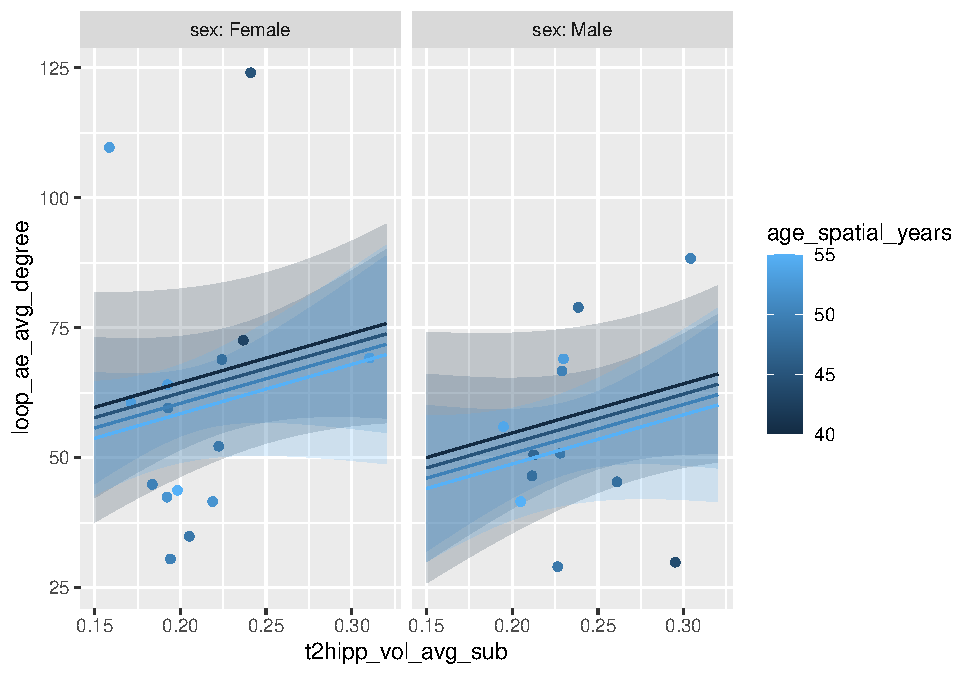
\includegraphics{hippocampal_subfield_files/figure-latex/Avg SUB + avg angular error MLR-1.pdf}
\vspace{1cm}

\newpage
\subsubsection{rad3}

\paragraph{CA1}

~ \vspace{1cm}

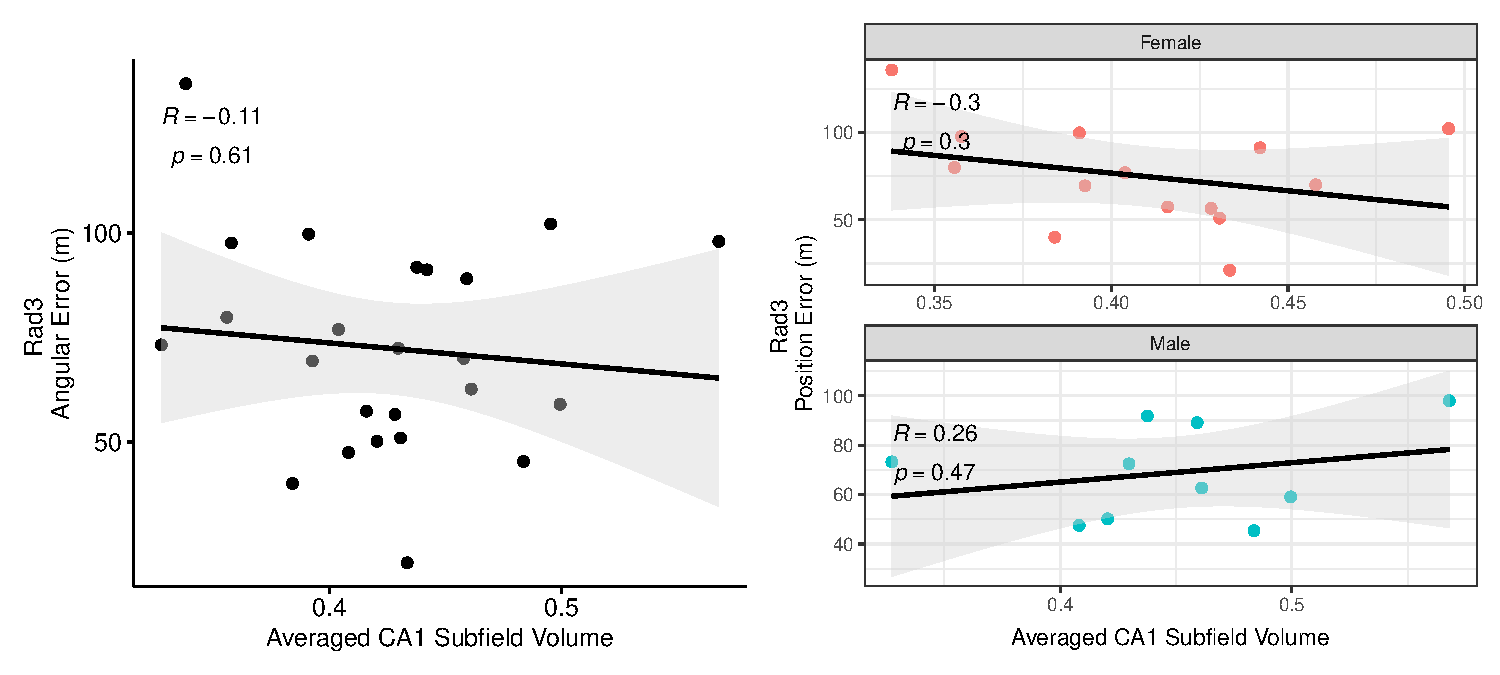
\includegraphics{hippocampal_subfield_files/figure-latex/unnamed-chunk-8-1.pdf}

\vspace{1cm}

Running multiple linear regressions to see the effect of age and sex and
then plotting results

\begin{verbatim}
## 
## Call:
## lm(formula = loop_ae_rad3_degree ~ t2hipp_vol_avg_ca1 + age_spatial_years + 
##     sex, data = df)
## 
## Residuals:
##     Min      1Q  Median      3Q     Max 
## -52.982 -18.156  -1.588  20.583  58.394 
## 
## Coefficients:
##                     Estimate Std. Error t value Pr(>|t|)
## (Intercept)         87.91165  158.35101   0.555    0.585
## t2hipp_vol_avg_ca1 -33.97922  128.81707  -0.264    0.795
## age_spatial_years    0.01789    2.44357   0.007    0.994
## sexMale             -4.57715   12.08037  -0.379    0.709
## 
## Residual standard error: 26.92 on 20 degrees of freedom
##   (4 observations deleted due to missingness)
## Multiple R-squared:  0.01897,    Adjusted R-squared:  -0.1282 
## F-statistic: 0.1289 on 3 and 20 DF,  p-value: 0.9418
\end{verbatim}

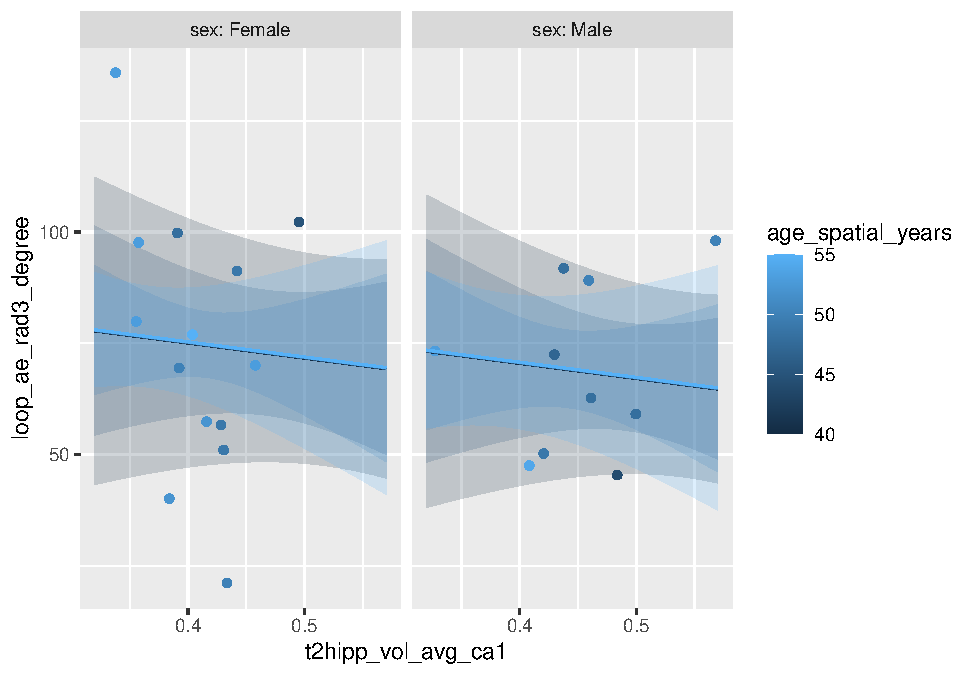
\includegraphics{hippocampal_subfield_files/figure-latex/Avg CA1 + rad3 angular errorMLR-1.pdf}
\vspace{1cm}

\paragraph{CA2/3}

~ \vspace{1cm}

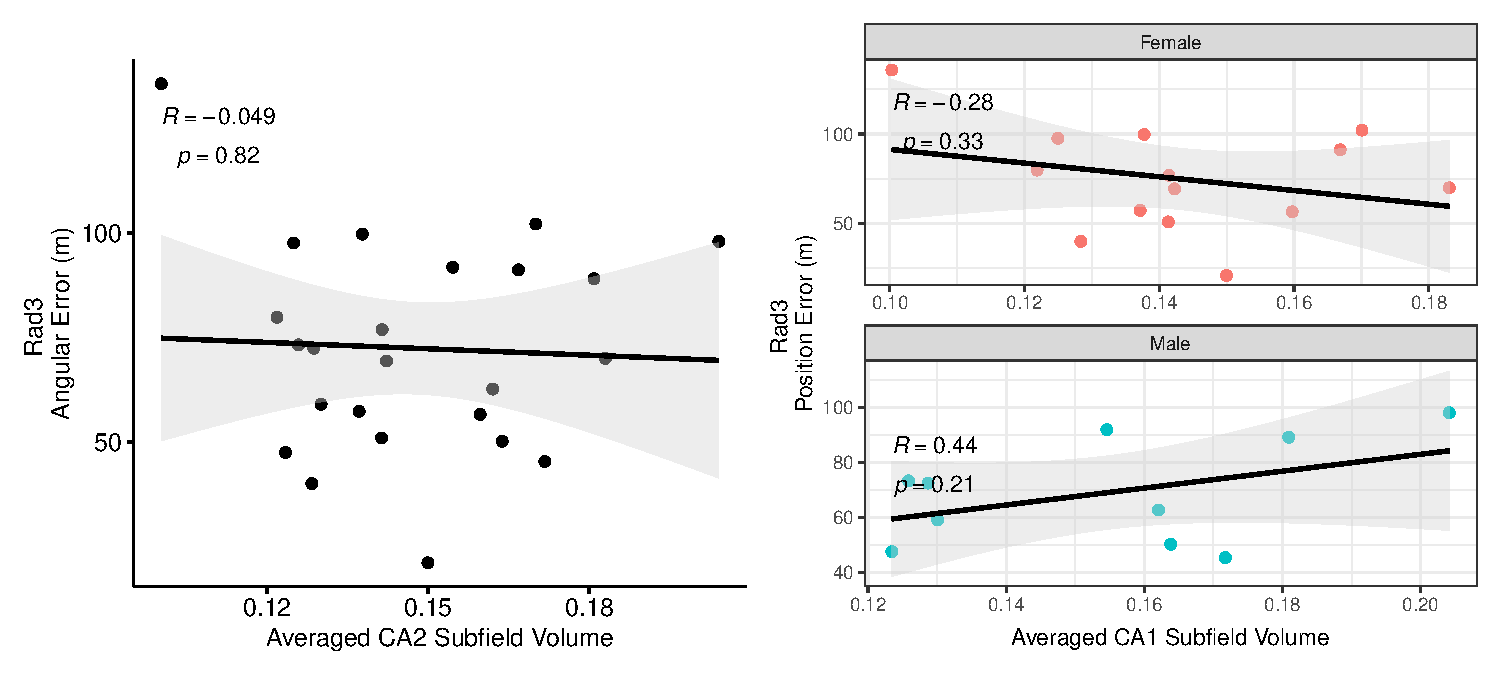
\includegraphics{hippocampal_subfield_files/figure-latex/unnamed-chunk-9-1.pdf}

\vspace{1cm}

Running multiple linear regressions to see the effect of age and sex and
then plotting results

\begin{verbatim}
## 
## Call:
## lm(formula = loop_ae_rad3_degree ~ t2hipp_vol_avg_ca23 + age_spatial_years + 
##     sex, data = df)
## 
## Residuals:
##     Min      1Q  Median      3Q     Max 
## -53.511 -18.167  -2.319  20.532  59.742 
## 
## Coefficients:
##                     Estimate Std. Error t value Pr(>|t|)
## (Intercept)          59.6795   133.0222   0.449    0.659
## t2hipp_vol_avg_ca23  -9.0246   257.8952  -0.035    0.972
## age_spatial_years     0.3256     2.2524   0.145    0.887
## sexMale              -5.3319    11.8003  -0.452    0.656
## 
## Residual standard error: 26.97 on 20 degrees of freedom
##   (4 observations deleted due to missingness)
## Multiple R-squared:  0.01562,    Adjusted R-squared:  -0.132 
## F-statistic: 0.1058 on 3 and 20 DF,  p-value: 0.9557
\end{verbatim}

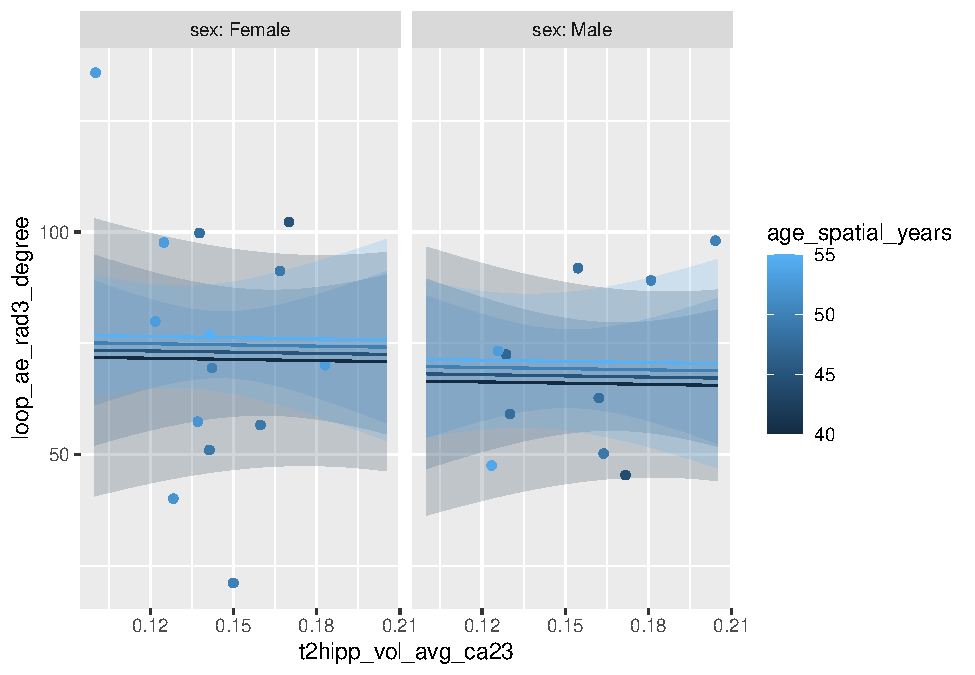
\includegraphics{hippocampal_subfield_files/figure-latex/avg CA2/3 + rad3 angular errorMLR-1.pdf}
\vspace{1cm}

\newpage
\paragraph{DG}

~ \vspace{1cm}

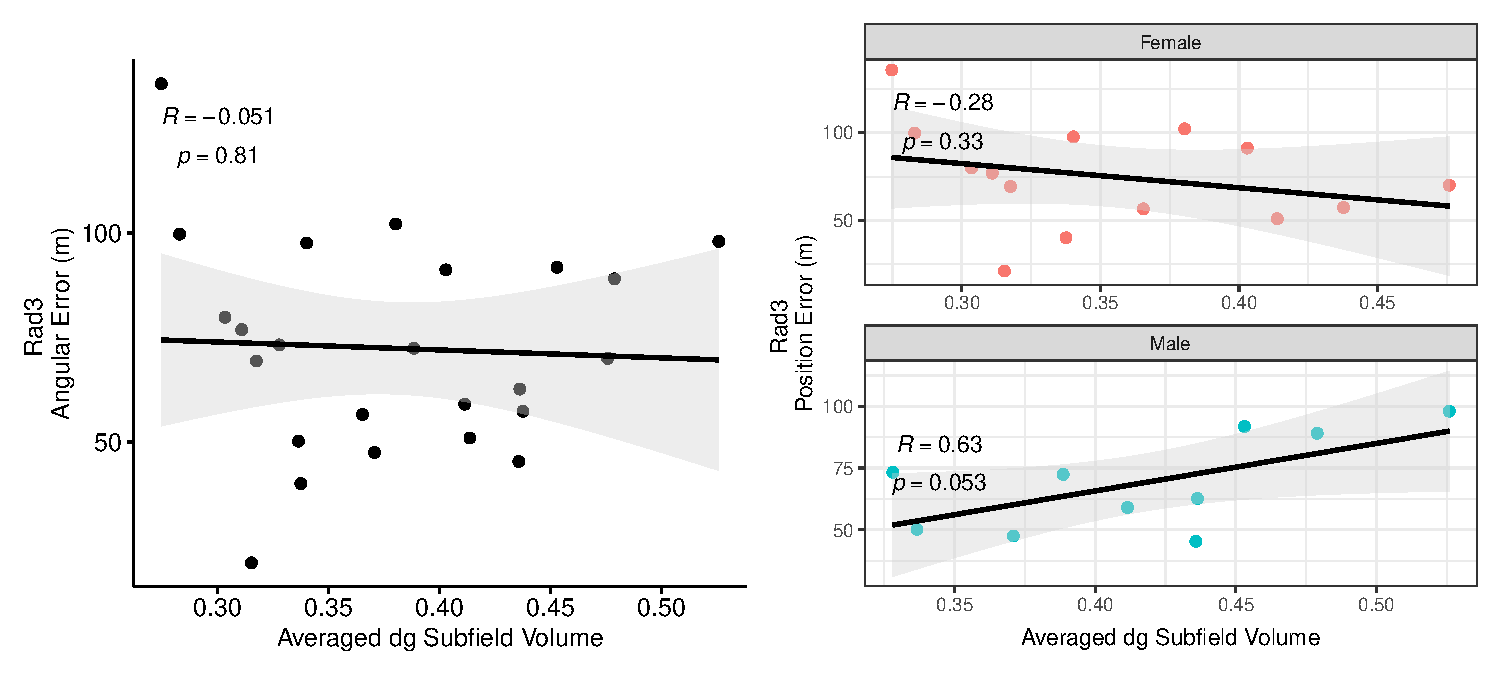
\includegraphics{hippocampal_subfield_files/figure-latex/unnamed-chunk-10-1.pdf}

\vspace{1cm}

Running multiple linear regressions to see the effect of age and sex and
then plotting results

\begin{verbatim}
## 
## Call:
## lm(formula = loop_ae_rad3_degree ~ t2hipp_vol_avg_dg + age_spatial_years + 
##     sex, data = df)
## 
## Residuals:
##     Min      1Q  Median      3Q     Max 
## -53.310 -18.320  -2.189  20.083  60.453 
## 
## Coefficients:
##                   Estimate Std. Error t value Pr(>|t|)
## (Intercept)        53.5843   120.0348   0.446    0.660
## t2hipp_vol_avg_dg   5.6223    95.7789   0.059    0.954
## age_spatial_years   0.3809     2.1303   0.179    0.860
## sexMale            -5.6911    12.8234  -0.444    0.662
## 
## Residual standard error: 26.97 on 20 degrees of freedom
##   (4 observations deleted due to missingness)
## Multiple R-squared:  0.01573,    Adjusted R-squared:  -0.1319 
## F-statistic: 0.1065 on 3 and 20 DF,  p-value: 0.9553
\end{verbatim}

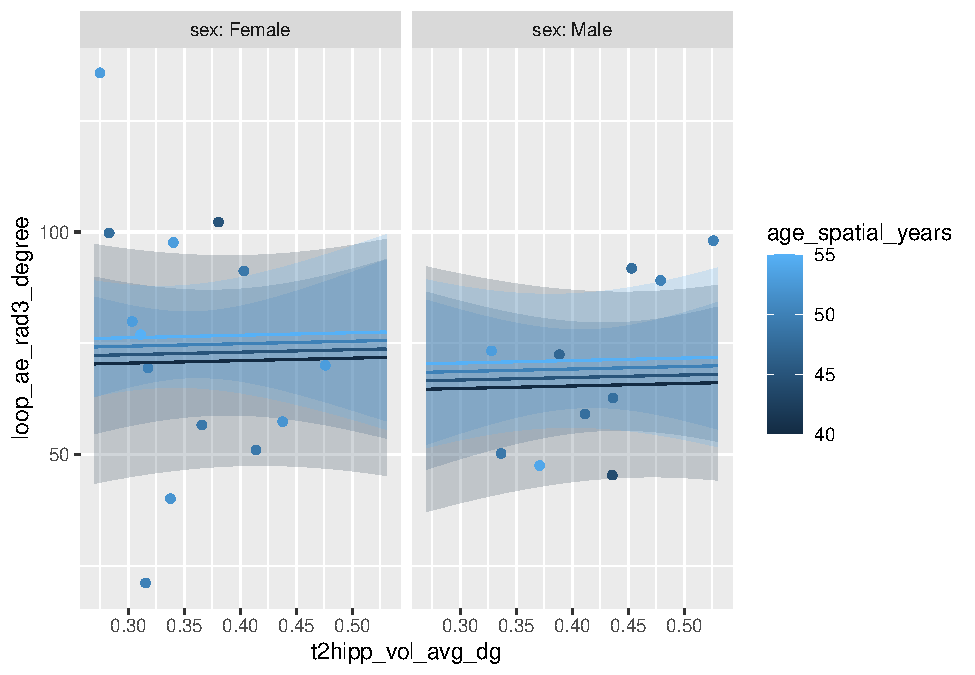
\includegraphics{hippocampal_subfield_files/figure-latex/AVG DG + rad3 angular errorMLR-1.pdf}
\vspace{1cm}

\paragraph{PHC}

~ \vspace{1cm}

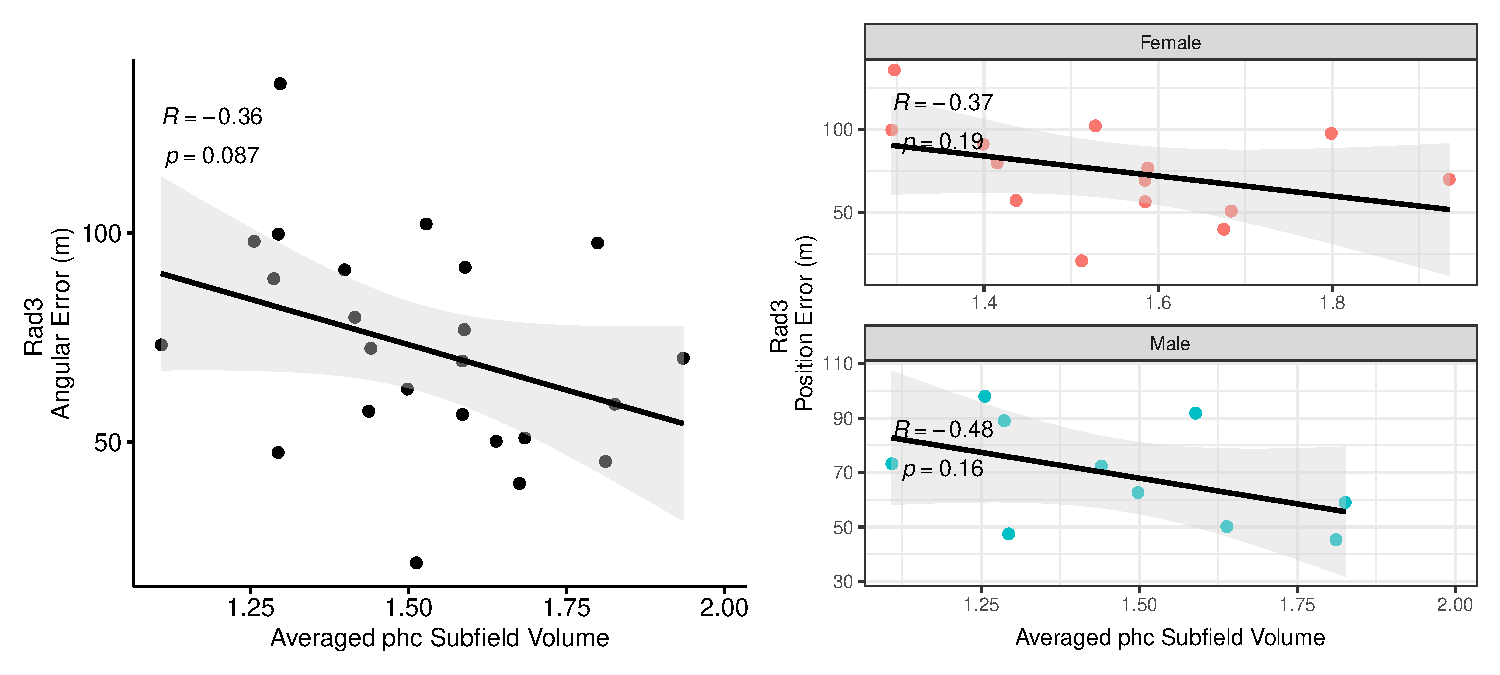
\includegraphics{hippocampal_subfield_files/figure-latex/unnamed-chunk-11-1.pdf}

\vspace{1cm}

Running multiple linear regressions to see the effect of age and sex and
then plotting results

\begin{verbatim}
## 
## Call:
## lm(formula = loop_ae_rad3_degree ~ t2hipp_vol_avg_phc + age_spatial_years + 
##     sex, data = df)
## 
## Residuals:
##     Min      1Q  Median      3Q     Max 
## -56.350 -13.091  -0.053  12.407  49.480 
## 
## Coefficients:
##                    Estimate Std. Error t value Pr(>|t|)  
## (Intercept)        185.6631   118.6032   1.565   0.1332  
## t2hipp_vol_avg_phc -50.1303    26.2231  -1.912   0.0704 .
## age_spatial_years   -0.6482     1.9882  -0.326   0.7478  
## sexMale            -10.9588    11.1530  -0.983   0.3375  
## ---
## Signif. codes:  0 '***' 0.001 '**' 0.01 '*' 0.05 '.' 0.1 ' ' 1
## 
## Residual standard error: 24.8 on 20 degrees of freedom
##   (4 observations deleted due to missingness)
## Multiple R-squared:  0.1677, Adjusted R-squared:  0.0428 
## F-statistic: 1.343 on 3 and 20 DF,  p-value: 0.2887
\end{verbatim}

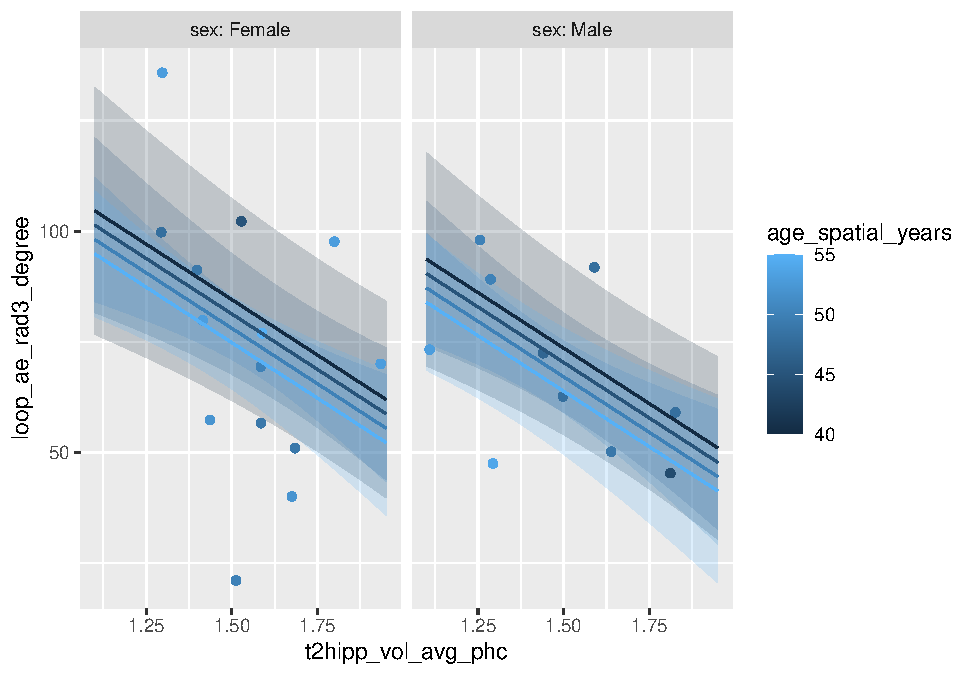
\includegraphics{hippocampal_subfield_files/figure-latex/Avg PHC + rad3 angular errorMLR-1.pdf}
\vspace{1cm}

\newpage
\paragraph{PRC}

~ \vspace{1cm}

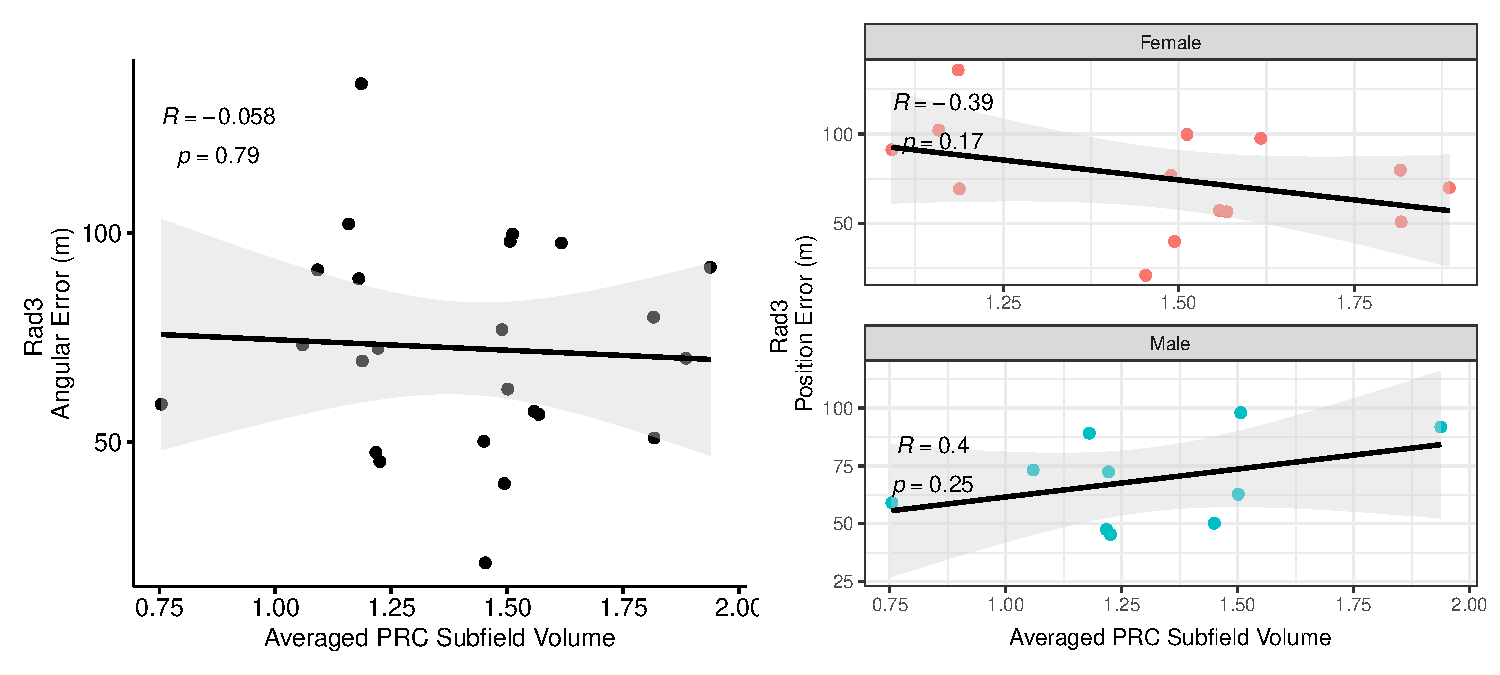
\includegraphics{hippocampal_subfield_files/figure-latex/unnamed-chunk-12-1.pdf}

\vspace{1cm}

Running multiple linear regressions to see the effect of age and sex and
then plotting results

\begin{verbatim}
## 
## Call:
## lm(formula = loop_ae_rad3_degree ~ t2hipp_vol_avg_prc + age_spatial_years + 
##     sex, data = df)
## 
## Residuals:
##     Min      1Q  Median      3Q     Max 
## -53.787 -17.322  -1.064  19.579  56.773 
## 
## Coefficients:
##                    Estimate Std. Error t value Pr(>|t|)
## (Intercept)         64.5652   106.7372   0.605    0.552
## t2hipp_vol_avg_prc  -9.8784    20.4537  -0.483    0.634
## age_spatial_years    0.4934     2.0930   0.236    0.816
## sexMale             -6.9556    12.0860  -0.576    0.571
## 
## Residual standard error: 26.81 on 20 degrees of freedom
##   (4 observations deleted due to missingness)
## Multiple R-squared:  0.02691,    Adjusted R-squared:  -0.1191 
## F-statistic: 0.1843 on 3 and 20 DF,  p-value: 0.9058
\end{verbatim}

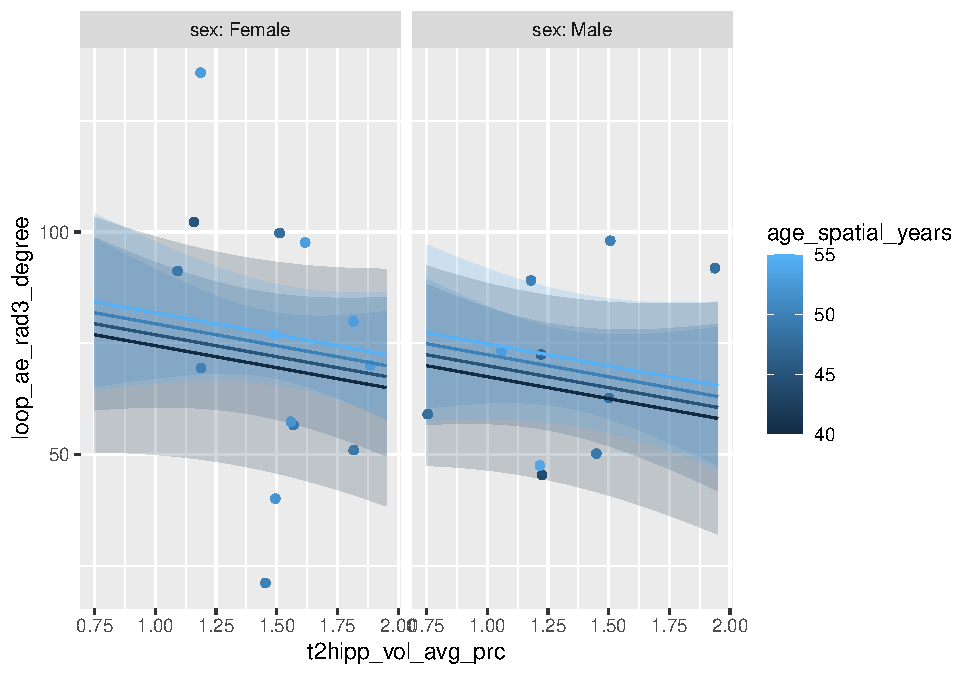
\includegraphics{hippocampal_subfield_files/figure-latex/Avg PRC + rad3 angular errorMLR-1.pdf}
\vspace{1cm}

\paragraph{ERC}

~ \vspace{1cm}

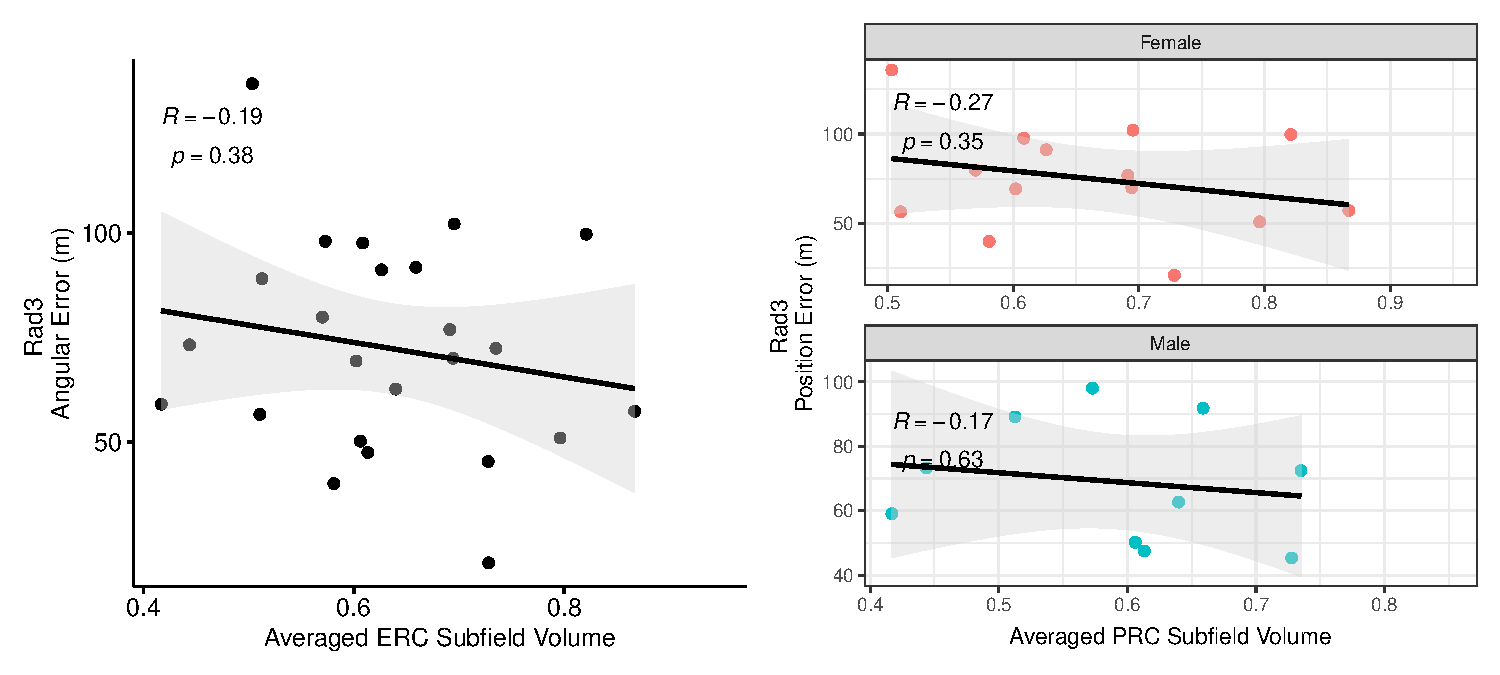
\includegraphics{hippocampal_subfield_files/figure-latex/unnamed-chunk-13-1.pdf}

\vspace{1cm}

Running multiple linear regressions to see the effect of age and sex and
then plotting results

\begin{verbatim}
## 
## Call:
## lm(formula = loop_ae_rad3_degree ~ t2hipp_vol_avg_erc + age_spatial_years + 
##     sex, data = df)
## 
## Residuals:
##     Min      1Q  Median      3Q     Max 
## -50.386 -17.883  -2.328  16.995  52.388 
## 
## Coefficients:
##                    Estimate Std. Error t value Pr(>|t|)
## (Intercept)        139.0132   127.2092   1.093    0.287
## t2hipp_vol_avg_erc -59.4390    53.9482  -1.102    0.284
## age_spatial_years   -0.4849     2.1638  -0.224    0.825
## sexMale            -11.0335    12.4704  -0.885    0.387
## 
## Residual standard error: 26.19 on 20 degrees of freedom
##   (4 observations deleted due to missingness)
## Multiple R-squared:  0.07189,    Adjusted R-squared:  -0.06733 
## F-statistic: 0.5164 on 3 and 20 DF,  p-value: 0.6757
\end{verbatim}

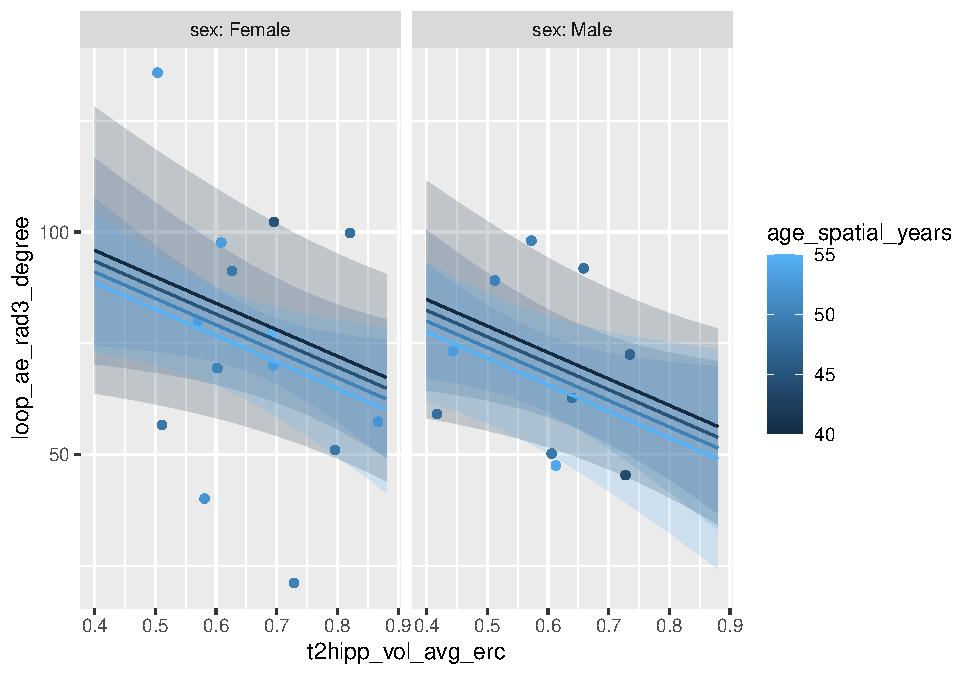
\includegraphics{hippocampal_subfield_files/figure-latex/Avg ERC + rad3 angular errorMLR-1.pdf}
\vspace{1cm}

\newpage
\paragraph{SUB}

~ \vspace{1cm}

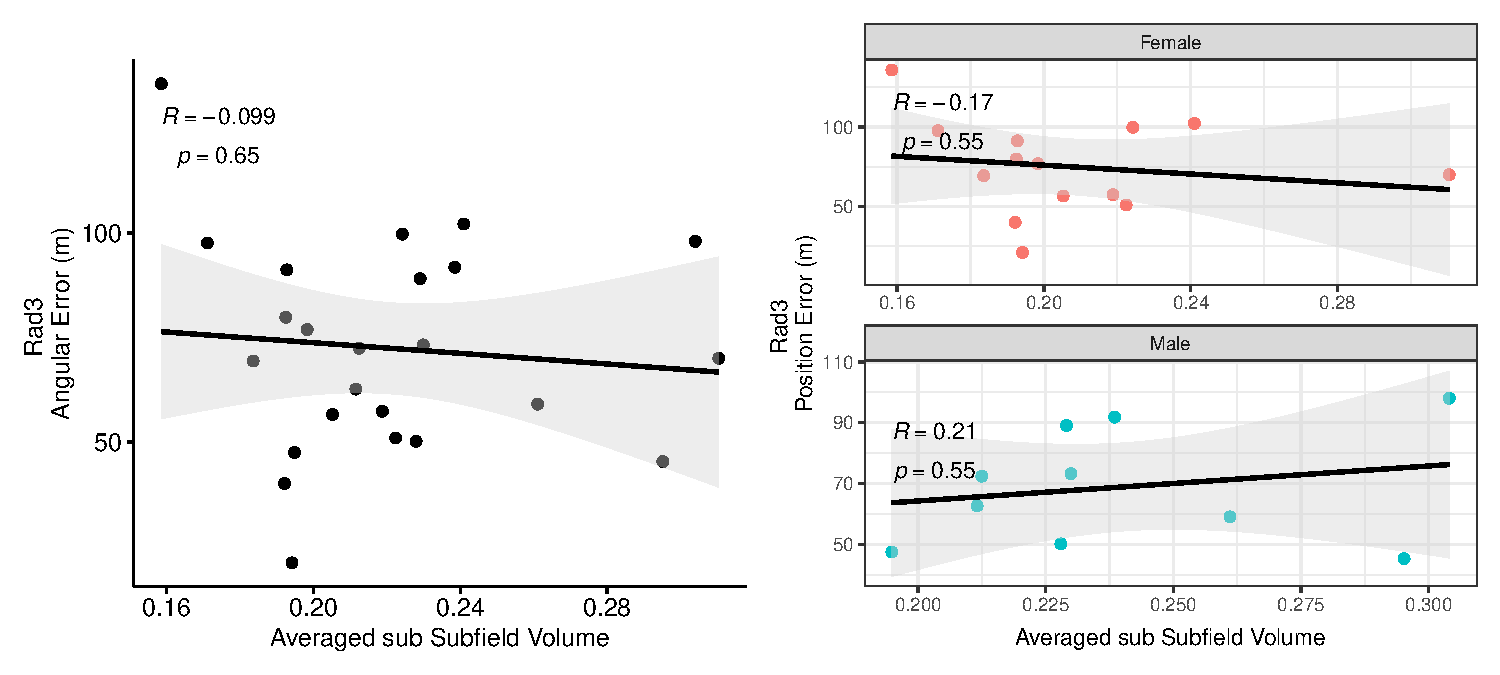
\includegraphics{hippocampal_subfield_files/figure-latex/unnamed-chunk-14-1.pdf}

\vspace{1cm}

Running multiple linear regressions to see the effect of age and sex and
then plotting results

\begin{verbatim}
## 
## Call:
## lm(formula = loop_ae_rad3_degree ~ t2hipp_vol_avg_sub + age_spatial_years + 
##     sex, data = df)
## 
## Residuals:
##     Min      1Q  Median      3Q     Max 
## -54.092 -18.278  -0.619  19.939  58.744 
## 
## Coefficients:
##                    Estimate Std. Error t value Pr(>|t|)
## (Intercept)         70.4116   126.0350   0.559    0.583
## t2hipp_vol_avg_sub -32.9302   165.6601  -0.199    0.844
## age_spatial_years    0.2234     2.1867   0.102    0.920
## sexMale             -4.5207    12.4757  -0.362    0.721
## 
## Residual standard error: 26.94 on 20 degrees of freedom
##   (4 observations deleted due to missingness)
## Multiple R-squared:  0.0175, Adjusted R-squared:  -0.1299 
## F-statistic: 0.1187 on 3 and 20 DF,  p-value: 0.948
\end{verbatim}

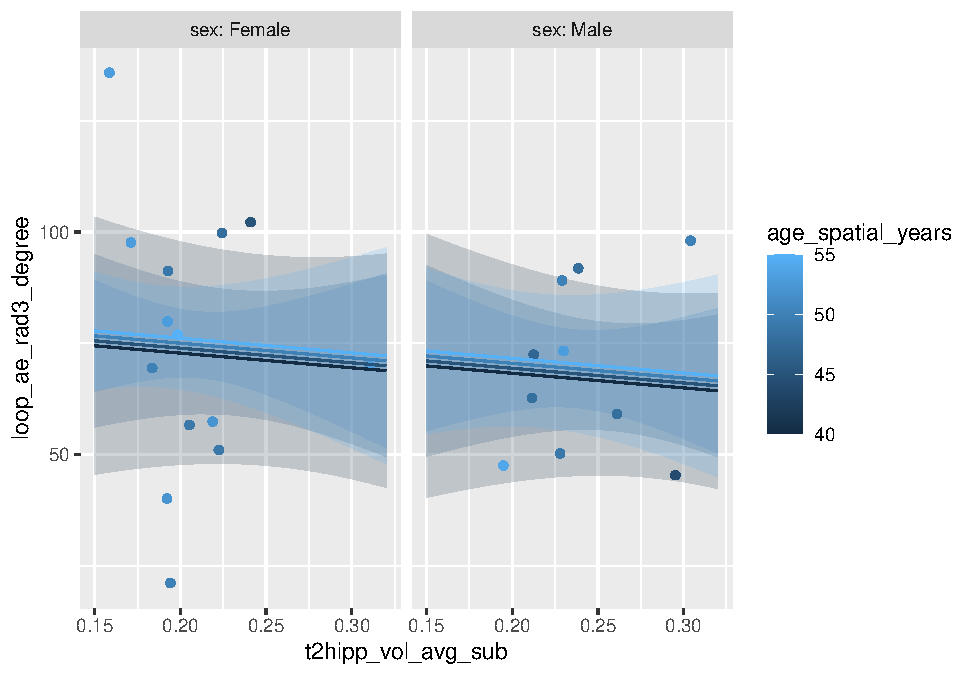
\includegraphics{hippocampal_subfield_files/figure-latex/Avg SUB + rad3 angular errorMLR-1.pdf}
\vspace{1cm}

\newpage

\subsection{Degrees Traveled Error}
\vspace{1cm}

\subsubsection{Average}

\paragraph{CA1}

~ \vspace{1cm}

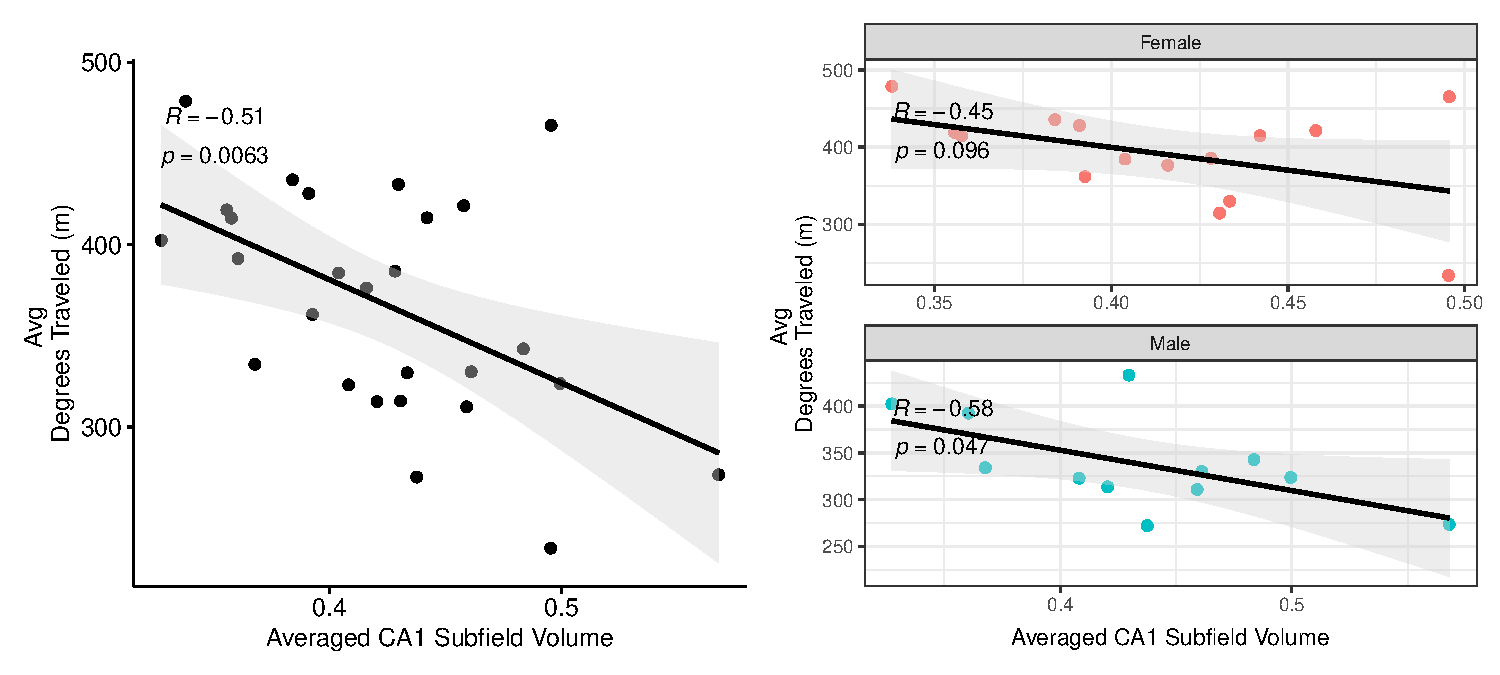
\includegraphics{hippocampal_subfield_files/figure-latex/unnamed-chunk-15-1.pdf}

\vspace{1cm}

Running multiple linear regressions to see the effect of age and sex and
then plotting results

\begin{verbatim}
## 
## Call:
## lm(formula = loop_de_avg_degree ~ t2hipp_vol_avg_ca1 + age_spatial_years + 
##     sex, data = df)
## 
## Residuals:
##      Min       1Q   Median       3Q      Max 
## -121.653  -27.648    0.156   22.438  107.166 
## 
## Coefficients:
##                    Estimate Std. Error t value Pr(>|t|)  
## (Intercept)         701.593    273.313   2.567   0.0172 *
## t2hipp_vol_avg_ca1 -550.335    230.701  -2.385   0.0257 *
## age_spatial_years    -1.641      4.064  -0.404   0.6901  
## sexMale             -42.948     20.398  -2.106   0.0464 *
## ---
## Signif. codes:  0 '***' 0.001 '**' 0.01 '*' 0.05 '.' 0.1 ' ' 1
## 
## Residual standard error: 51.76 on 23 degrees of freedom
##   (1 observation deleted due to missingness)
## Multiple R-squared:  0.3851, Adjusted R-squared:  0.3049 
## F-statistic: 4.802 on 3 and 23 DF,  p-value: 0.009683
\end{verbatim}

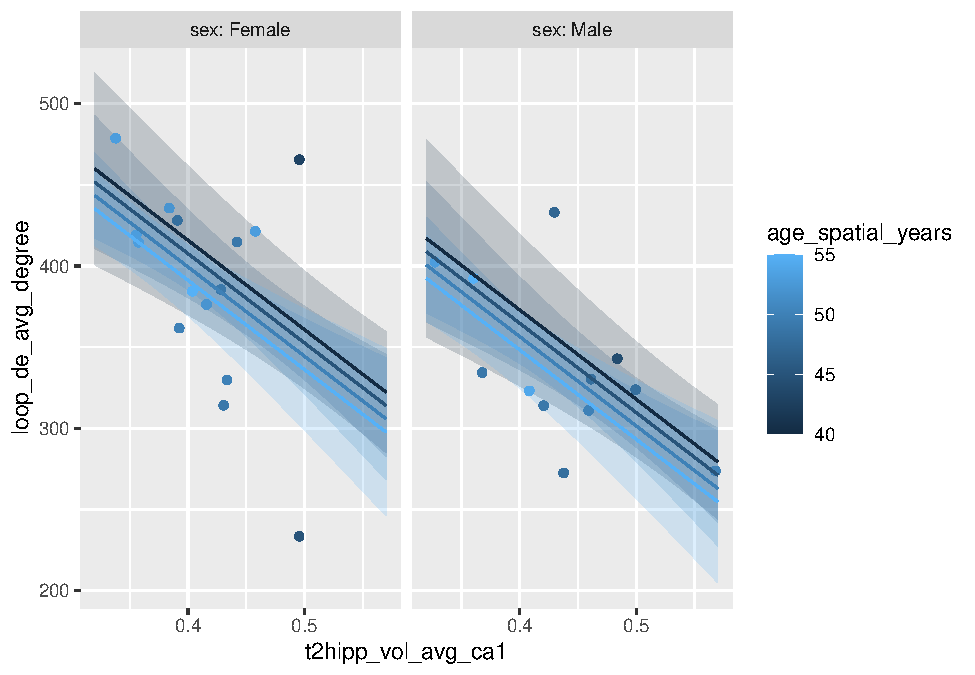
\includegraphics{hippocampal_subfield_files/figure-latex/Avg CA1 + AVG Degrees Traveled MLR-1.pdf}
\vspace{1cm}

\paragraph{CA2/3}

~ \vspace{1cm}

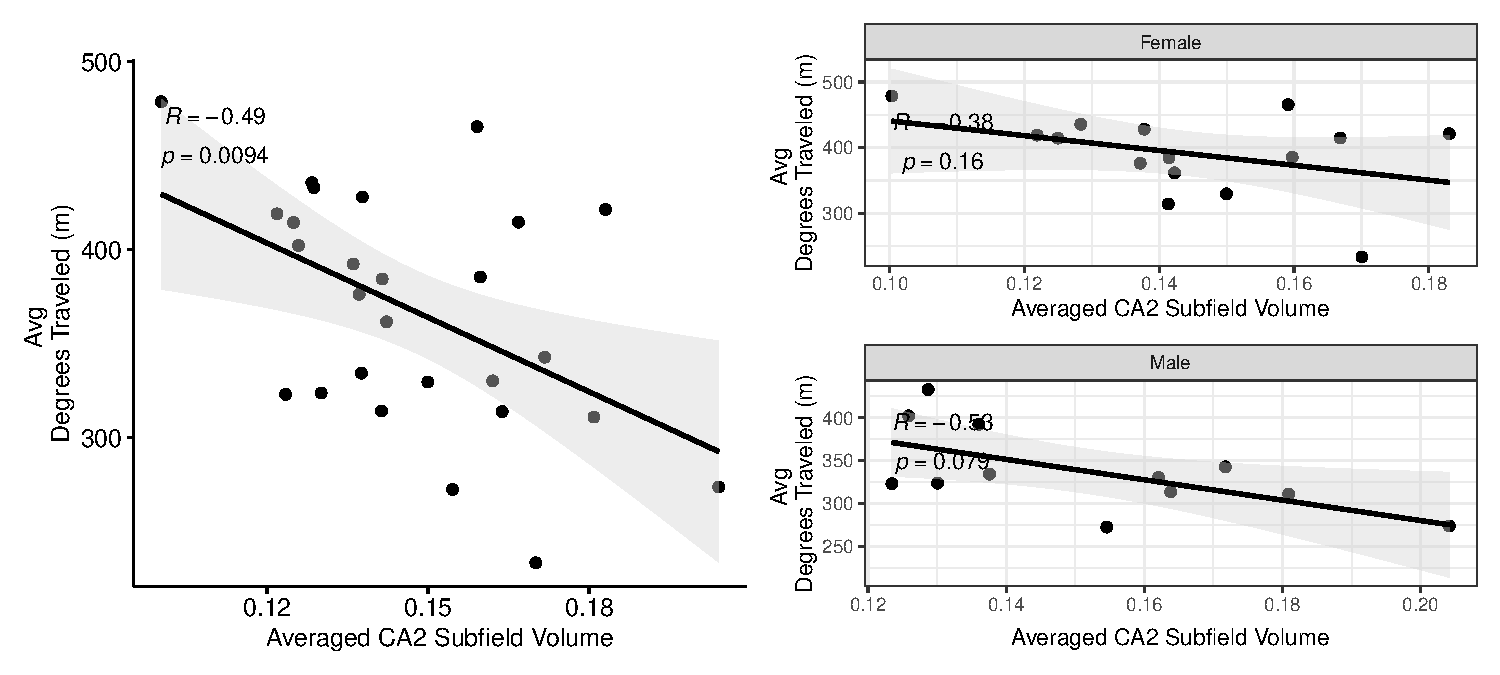
\includegraphics{hippocampal_subfield_files/figure-latex/unnamed-chunk-16-1.pdf}

\paragraph{DG}

~ \vspace{1cm}

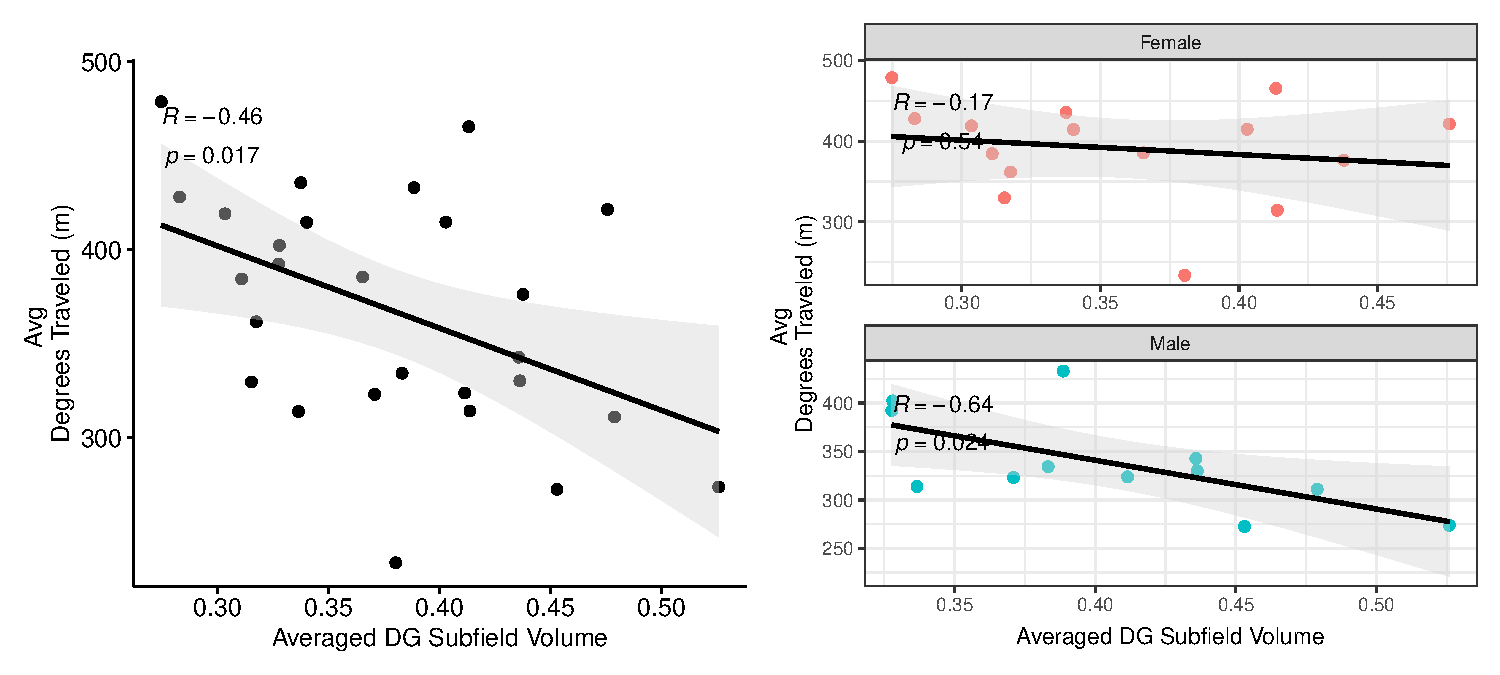
\includegraphics{hippocampal_subfield_files/figure-latex/unnamed-chunk-17-1.pdf}

\paragraph{ERC}

~ \vspace{1cm}

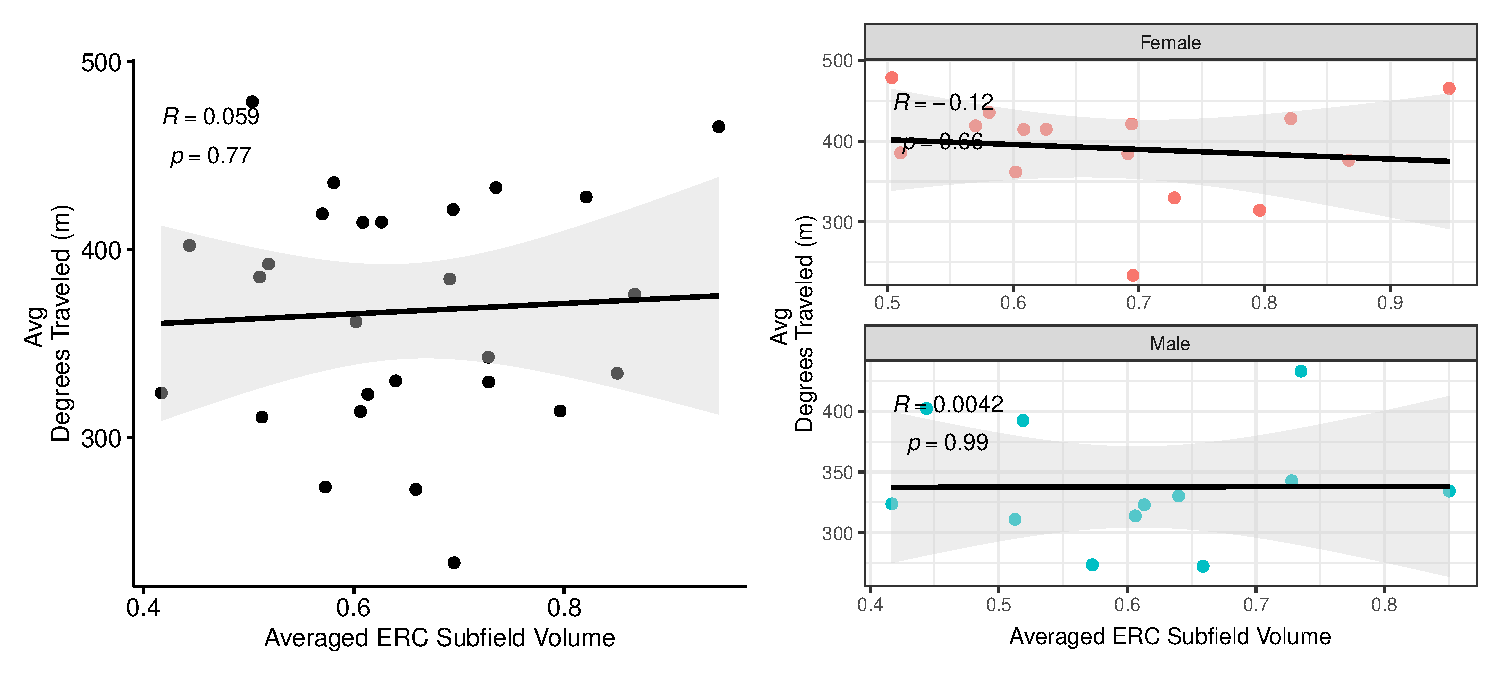
\includegraphics{hippocampal_subfield_files/figure-latex/unnamed-chunk-18-1.pdf}

\paragraph{PHC}

~ \vspace{1cm}

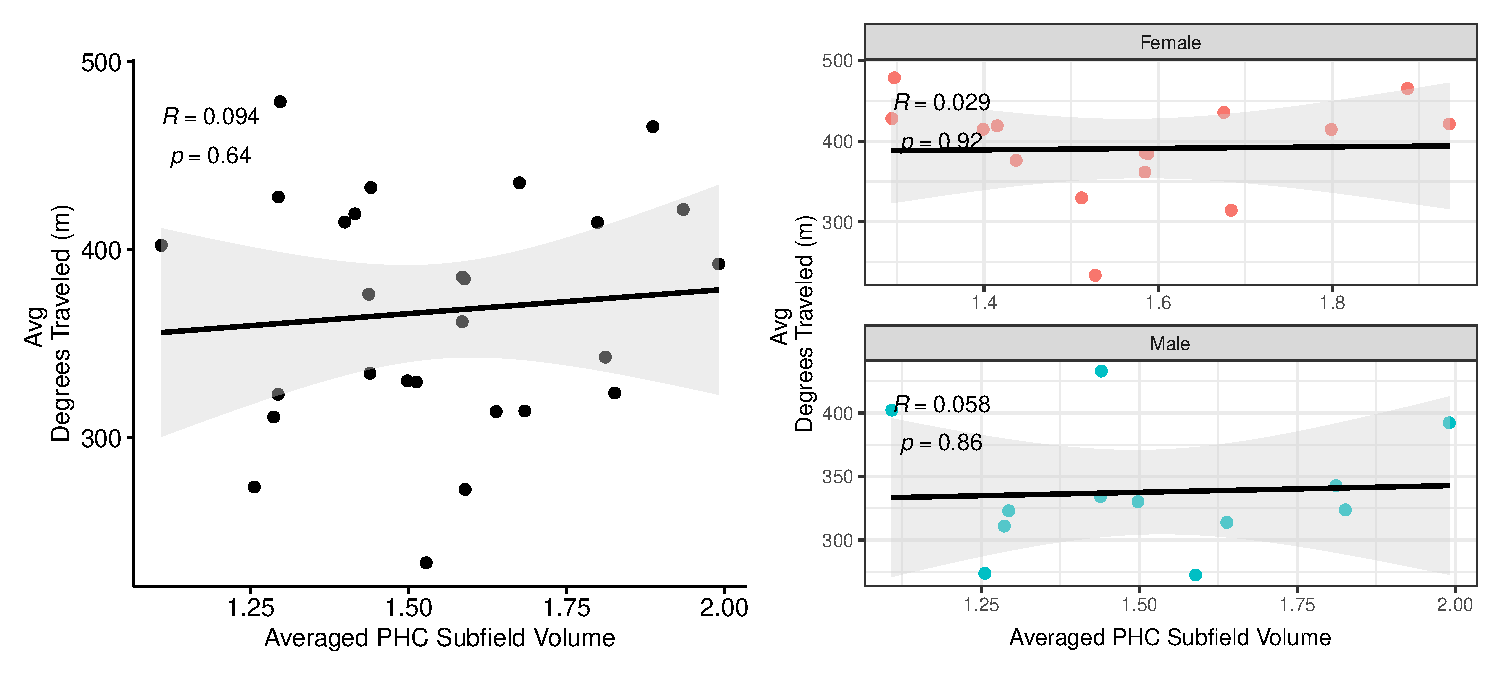
\includegraphics{hippocampal_subfield_files/figure-latex/unnamed-chunk-19-1.pdf}

\subsubsection{Rad3}

\end{document}
